\chapter{EM Algorithms for Text Processing}
\label{chapter6}

Until the end of the 1980s, text processing systems tended to rely on
large numbers of manually written rules to analyze, annotate, and
transform text input, usually in a deterministic way.  This rule-based
approach can be appealing:\ a system's behavior can generally be
understood and predicted precisely, and, when errors surface, they can
be corrected by writing new rules or refining old ones. However,
rule-based systems suffer from a number of serious problems.  They are
brittle with respect to the natural variation found in language, and
developing systems that can deal with inputs from diverse domains is
very labor intensive.  Furthermore, when these systems fail, they
often do so catastrophically, unable to offer even a ``best guess'' as
to what the desired analysis of the input might be.

In the last 20 years, the rule-based approach has largely been
abandoned in favor of more data-driven methods, where the ``rules''
for processing the input are inferred automatically from large corpora
of examples, called \emph{training data}.  The basic strategy of the
data-driven approach is to start with a processing algorithm capable
of capturing how any instance of the \emph{kinds} of inputs (e.g.,
sentences or emails) can relate to any instance of the kinds of
outputs that the final system should produce (e.g., the syntactic
structure of the sentence or a classification of the email as spam).
At this stage, the system can be thought of as having the potential to
produce any output for any input, but they are not distinguished in
any way.  Next, a \emph{learning algorithm} is applied which refines
this process based on the training data---generally attempting to make
the model perform as well as possible at predicting the examples in
the training data.  The learning process, which often involves
iterative algorithms, typically consists of activities like ranking
rules, instantiating the content of rule templates, or determining
parameter settings for a given model. This is known as \emph{machine
  learning}, an active area of research.

Data-driven approaches have turned out to have several benefits over
rule-based approaches to system development.  Since data-driven
systems can be trained using examples of the kind that they will
eventually be used to process, they tend to deal with the complexities
found in real data more robustly than rule-based systems do.  Second,
developing training data tends to be far less expensive than
developing rules.  For some applications, significant quantities of
training data may even exist for independent reasons (e.g.,
translations of text into multiple languages are created by authors
wishing to reach an audience speaking different languages, not because
they are generating training data for a data-driven machine
translation system).  These advantages come at the cost of systems
that often behave internally quite differently than a human-engineered
system.  As a result, correcting errors that the trained system makes
can be quite challenging.

Data-driven information processing systems can be constructed using a
variety of mathematical techniques, but in this chapter we focus on
\emph{statistical models}, which probabilistically relate inputs from
an input set $\mathcal{X}$ (e.g., sentences, documents, etc.), which
are always \emph{observable}, to annotations from a set $\mathcal{Y}$,
which is the space of possible annotations or analyses that the system
should predict.  This model may take the form of either a \emph{joint
  model} $\Pr(x,y)$ which assigns a probability to every pair $\langle
x,y \rangle \in \mathcal{X} \times \mathcal{Y}$ or a \emph{conditional
  model} $\Pr(y|x)$, which assigns a probability to every $y \in
\mathcal{Y}$, given an $x \in \mathcal{X}$. For example, to create a
statistical spam detection system, we might have
$\mathcal{Y}=\{\textsc{Spam},\textsc{NotSpam}\}$ and $\mathcal{X}$ be
the set of all possible email messages.  For machine translation,
$\mathcal{X}$ might be the set of Arabic sentences and $\mathcal{Y}$
the set of English sentences.\footnote{In this chapter, we will
  consider discrete models only. They tend to be sufficient for text
  processing, and their presentation is simpler than models with
  continuous densities.  It should be kept in mind that the sets
  $\mathcal{X}$ and $\mathcal{Y}$ may still be countably infinite.}

There are three closely related, but distinct challenges in
statistical text-processing.  The first is model selection.  This
entails selecting a representation of a joint or conditional
distribution over the desired $\mathcal{X}$ and $\mathcal{Y}$.  For a
problem where $\mathcal{X}$ and $\mathcal{Y}$ are very small, one
could imagine representing these probabilities in look-up tables.
However, for something like email classification or machine
translation, where the model space is infinite, the probabilities
cannot be represented directly, and must be computed algorithmically.
As an example of such models, we introduce \emph{hidden Markov models}
(HMMs), which define a joint distribution over sequences of inputs and
sequences of annotations.  The second challenge is \emph{parameter
  estimation} or \emph{learning}, which involves the application of a
optimization algorithm and training criterion to select the parameters
of the model to optimize the model's performance (with respect to the
given training criterion) on the training data.\footnote{We restrict
  our discussion in this chapter to models with finite numbers of
  parameters and where the learning process refers to setting those
  parameters. Inference in and learning of so-called
  \emph{nonparameteric models}, which have an infinite number of
  parameters and have become important statistical models for text
  processing in recent years, is beyond the scope of this chapter.}
The parameters of a statistical model are the values used to compute
the probability of some event described by the model.  In this chapter
we will focus on one particularly simple training criterion for
parameter estimation, \emph{maximum likelihood estimation}, which says
to select the parameters that make the training data most probable
under the model, and one learning algorithm that attempts to meet this
criterion, called expectation maximization (EM).  The final challenge
for statistical modeling is the problem of \emph{decoding}, or, given
some $x$, using the model to select an annotation $y$.  One very
common strategy is to select $y$ according to the following criterion:

\begin{equation}
y^* = \arg \max_{y \in \mathcal{Y}} \Pr(y | x)
\end{equation}
In a conditional (or \emph{direct}) model, this is a straightforward search for the best $y$ under the model.  In a joint model, the search is also straightforward, on account of the definition of conditional probability:
\begin{equation}
y^* = \arg \max_{y \in \mathcal{Y}} \Pr(y|x) = \arg \max_{y \in \mathcal{Y}} \frac{\Pr(x,y)}{\sum_{y'}\Pr(x,y')} = \arg \max_{y \in \mathcal{Y}} \Pr(x,y) 
\end{equation}

\noindent The specific form that the search takes will depend on how
the model is represented.  Our focus in this chapter will primarily be
on the second problem:\ learning parameters for models, but we will
touch on the third problem as well.

Machine learning is often categorized as either \emph{supervised} or
\emph{unsupervised}.  Supervised learning of statistical models simply
means that the model parameters are estimated from training data
consisting of pairs of inputs and annotations, that is $\mathcal{Z} =
\left\langle \langle x_1,y_1 \rangle , \langle x_2,y_2 \rangle ,
\ldots \right\rangle$ where $\langle x_i, y_i \rangle \in \mathcal{X}
\times \mathcal{Y}$ and $y_i$ is the \emph{gold standard} (i.e.,
correct) annotation of $x_i$.  While supervised models often attain
quite good performance, they are often uneconomical to use, since the
training data requires each object that is to be classified (to pick a
specific task), $x_i$ to be paired with its correct label, $y_i$.  In
many cases, these gold standard training labels must be generated by a
process of \emph{expert annotation}, meaning that each $x_i$ must be
manually labeled by a trained individual.  Even when the annotation
task is quite simple for people to carry out (e.g., in the case of
spam detection), the number of potential examples that could be
classified (representing a subset of $\mathcal{X}$, which may of
course be infinite in size) will far exceed the amount of data that
can be annotated.  As the annotation task becomes more complicated
(e.g., when predicting more complex structures such as sequences of
labels or when the annotation task requires specialized expertise),
annotation becomes far more challenging.

Unsupervised learning, on the other hand, requires only that the
training data consist of a representative collection of objects that
should be annotated, that is $\mathcal{Z} = \left\langle x_1, x_2 ,
\ldots \right\rangle$ where $x_i \in \mathcal{X}$, but \emph{without}
any example annotations.  While it may at first seem counterintuitive
that meaningful annotations can be learned without any examples of the
desired annotations being given, the learning criteria and model
structure (which crucially define the space of possible annotations
$\mathcal{Y}$ and the process by which annotations relate to
observable inputs) make it possible to induce annotations by relying
on regularities in the unclassified training instances. While a
thorough discussion of unsupervised learning is beyond the scope of
this book, we focus on a particular class of algorithms---expectation
maximization (EM) algorithms---that can be used to learn the
parameters of a joint model $\Pr(x,y)$ from incomplete data (i.e.,
data where some of the variables in the model cannot be observed; in
the case of unsupervised learning, the $y_i$'s are unobserved).
Expectation maximization algorithms fit naturally into the MapReduce
paradigm, and are used to solve a number of problems of interest in
text processing.  Furthermore, these algorithms can be quite
computationally expensive, since they generally require repeated
evaluations of the training data.  MapReduce therefore provides an
opportunity not only to scale to larger amounts of data, but also to
improve efficiency bottlenecks at scales where non-parallel solutions
could be utilized.

This chapter is organized as follows.  In
Section~\ref{chapter6_intro}, we describe maximum likelihood
estimation for statistical models, show how this is generalized to
models where not all variables are observable, and then introduce
expectation maximization (EM).  We describe hidden Markov models
(HMMs) in Section~\ref{chapter6_hmms}, a very versatile class of
models that uses EM for parameter estimation.
Section~\ref{chapter6_mapreduce} discusses how EM algorithms can be
expressed in MapReduce, and then in
Section~\ref{chapter6_word_alignment} we look at a case study of word
alignment for statistical machine translation.
Section~\ref{chapter6_variants} examines similar algorithms that are
appropriate for supervised learning tasks.  This chapter concludes
with a summary and pointers to additional readings.

\section{Expectation Maximization}
\label{chapter6_intro}

Expectation maximization (EM) algorithms
\cite{Dempster_Laird_Rubin_1977} are a family of iterative
optimization algorithms for learning probability distributions from
incomplete data.  They are extensively used in statistical natural
language processing where one seeks to infer latent linguistic
structure from unannotated text.  To name just a few applications, EM
algorithms have been used to find part-of-speech sequences,
constituency and dependency trees, alignments between texts in
different languages, alignments between acoustic signals and their
transcriptions, as well as for numerous other clustering and structure
discovery problems.

Expectation maximization generalizes the principle of maximum
likelihood estimation to the case where the values of some variables
are unobserved (specifically, those characterizing the latent
structure that is sought).

\subsection{Maximum Likelihood Estimation}

Maximum likelihood estimation (MLE) is a criterion for fitting the
parameters $\theta$ of a statistical model to some given data
$\textbf{x}$.  Specifically, it says to select the parameter settings
$\theta^*$ such that the likelihood of observing the training data
given the model is maximized:
\begin{equation}
\theta^* = \arg \max_{\theta} \Pr(\textbf{X}=\textbf{x};\theta)
\end{equation}

To illustrate, consider the simple marble game shown in
Figure~\ref{chapter6_figure_plinko}.  In this game, a marble is
released at the position indicated by the black dot, and it bounces
down into one of the cups at the bottom of the board, being diverted
to the left or right by the peg (indicated by a triangle) in the
center.  Our task is to construct a model that predicts which cup the
ball will drop into.  A ``rule-based'' approach might be to take exact
measurements of the board and construct a physical model that we can
use to predict the behavior of the ball.  Given sophisticated enough
measurements, this could certainly lead to a very accurate model.
However, the construction of this model would be quite time consuming
and difficult.

A statistical approach, on the other hand, might be to assume that the
behavior of the marble in this game can be modeled using a Bernoulli
random variable $Y$ with parameter $p$.  That is, the value of the
random variable indicates whether path 0 or 1 is taken.  We also
define a random variable $X$ whose value is the label of the cup that
the marble ends up in; note that $X$ is deterministically related to
$Y$, so an observation of $X$ is equivalent to an observation of $Y$.

\begin{figure*}
\begin{center}
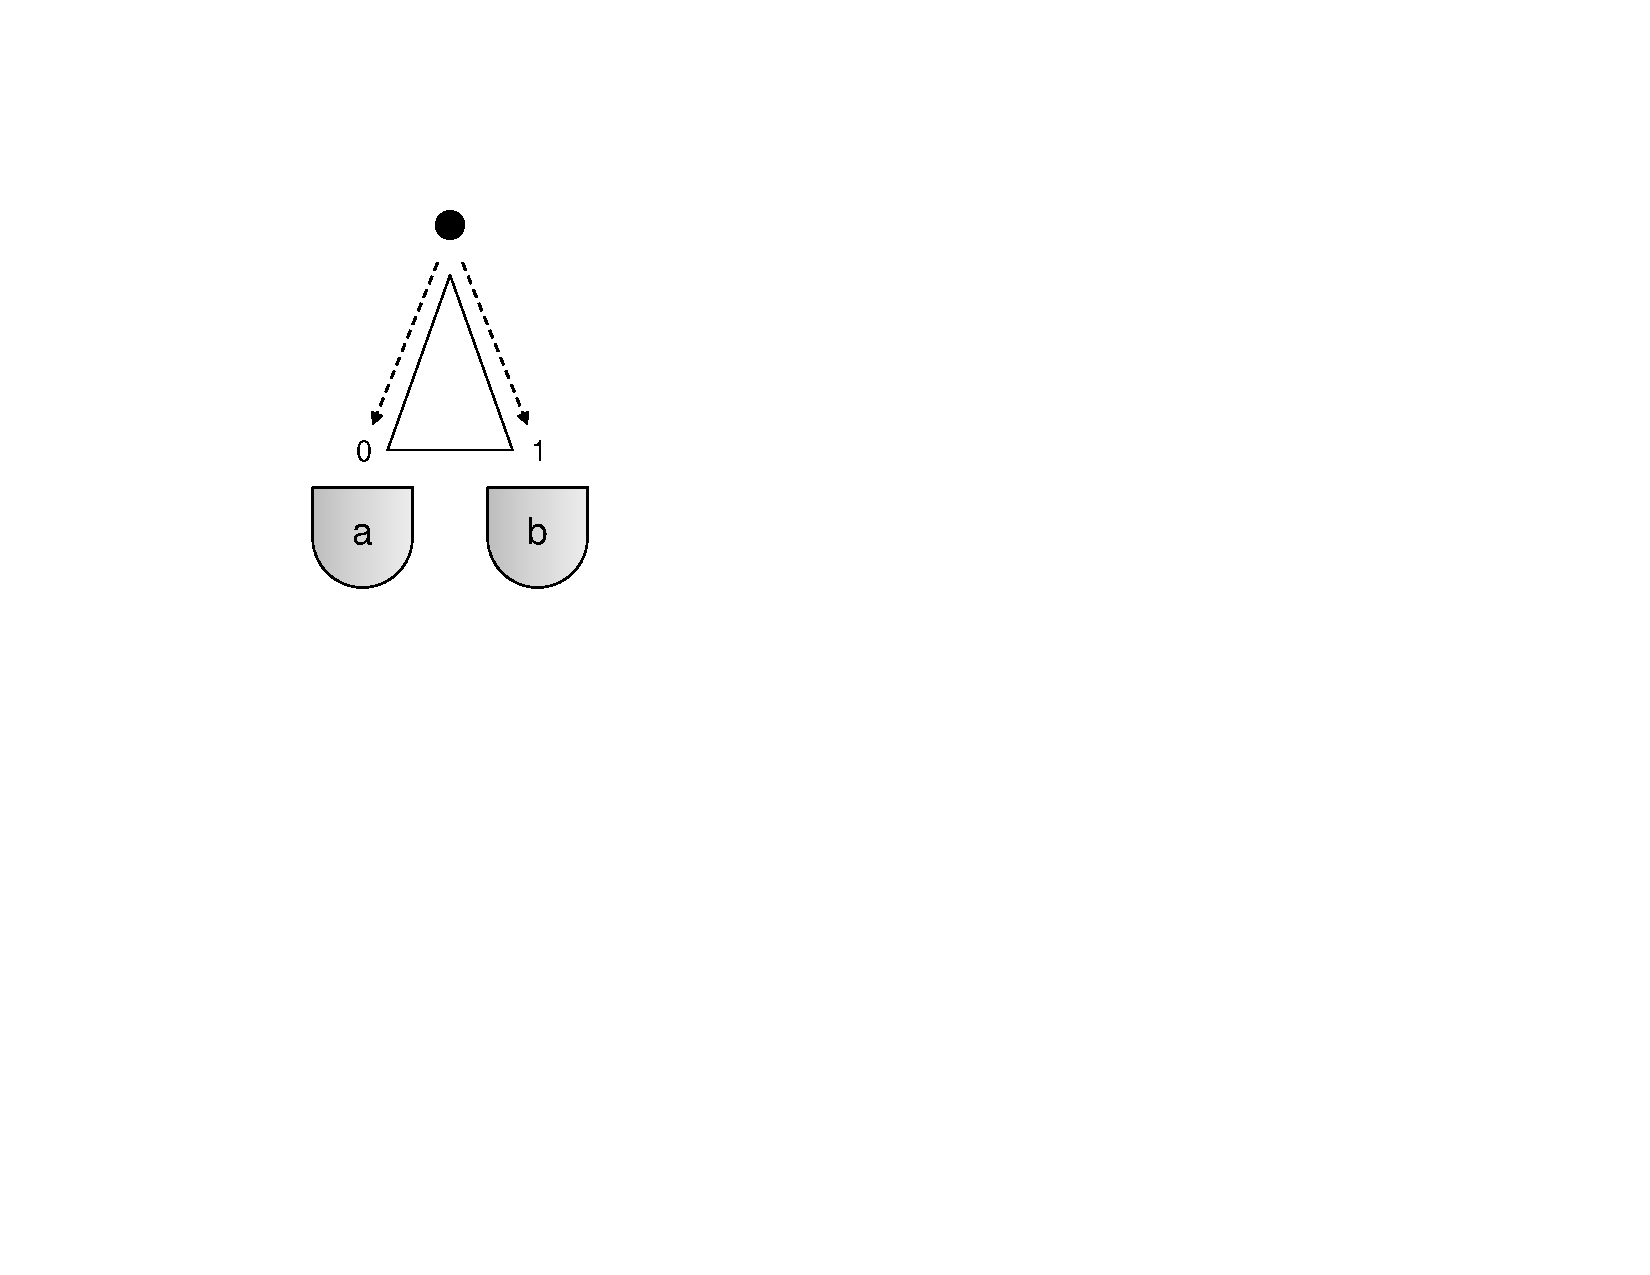
\includegraphics[scale=0.6]{figures/fig-ch6-em-marble1.pdf}
\end{center}\caption{A simple marble game where a released marble takes one of two possible paths.  This game can be modeled using a Bernoulli random variable with parameter $p$, which indicates the probability that the marble will go to the right when it hits the peg.}\label{chapter6_figure_plinko}
\end{figure*}

To estimate the parameter $p$ of the statistical model of our game, we
need some \emph{training data}, so we drop 10 marbles into the game
which end up in cups $\textbf{x} = \langle
b,b,b,a,b,b,b,b,b,a\rangle$.

What is the maximum likelihood estimate of $p$ given this data?  By
assuming that our samples are independent and identically distributed
(i.i.d.), we can write the likelihood of our data as
follows:\footnote{In this equation, $\delta$ is the Kroneker delta
  function which evaluates to 1 where its arguments are equal and 0
  otherwise.}
\begin{align}
\Pr(\textbf{x};p) & = \prod_{j=1}^{10} p^{\delta(x_j,a)}(1-p)^{\delta(x_j,b)} \\
&  = p^2 \cdot (1 - p)^8
\end{align}

\noindent Since $\log$ is a monotonically increasing function,
maximizing $\log \Pr(\textbf{x};p)$ will give us the desired result.
We can do this differentiating with respect to $p$ and finding where
the resulting expression equals 0:
\begin{align}
\frac{d \log \Pr(\textbf{x};p)}{dp} & = 0\\
\frac{d [ 2\cdot \log p + 8 \cdot \log (1-p) ]}{dp} & = 0 \\
\frac{2}{p} - \frac{8}{1-p} & = 0
\end{align}

\noindent Solving for $p$ yields $0.2$, which is the intuitive result.
Furthermore, it is straightforward to show that in $N$ trials where
$N_0$ marbles followed path 0 to cup $a$, and $N_1$ marbles followed
path 1 to cup $b$, the maximum likelihood estimate of $p$ is $N_1 /
(N_0 + N_1)$.

While this model only makes use of an approximation of the true
physical process at work when the marble interacts with the game
board, it is an empirical question whether the model works well enough
in practice to be useful.  Additionally, while a Bernoulli trial is an
extreme approximation of the physical process, if insufficient
resources were invested in building a physical model, the
approximation may perform better than the more complicated
``rule-based'' model.  This sort of dynamic is found often in text
processing problems:\ given enough data, astonishingly simple models
can outperform complex knowledge-intensive models that attempt to
simulate complicated processes.

\subsection{A Latent Variable Marble Game}
\label{chapter6_em_example}

To see where latent variables might come into play in modeling,
consider a more complicated variant of our marble game shown in
Figure~\ref{chapter6_figure_plinko2}.  This version consists of three
pegs that influence the marble's path, and the marble may end up in
one of three cups.  Note that both paths 1 and 2 lead to cup $b$.

\begin{figure*}[t]
\begin{center}
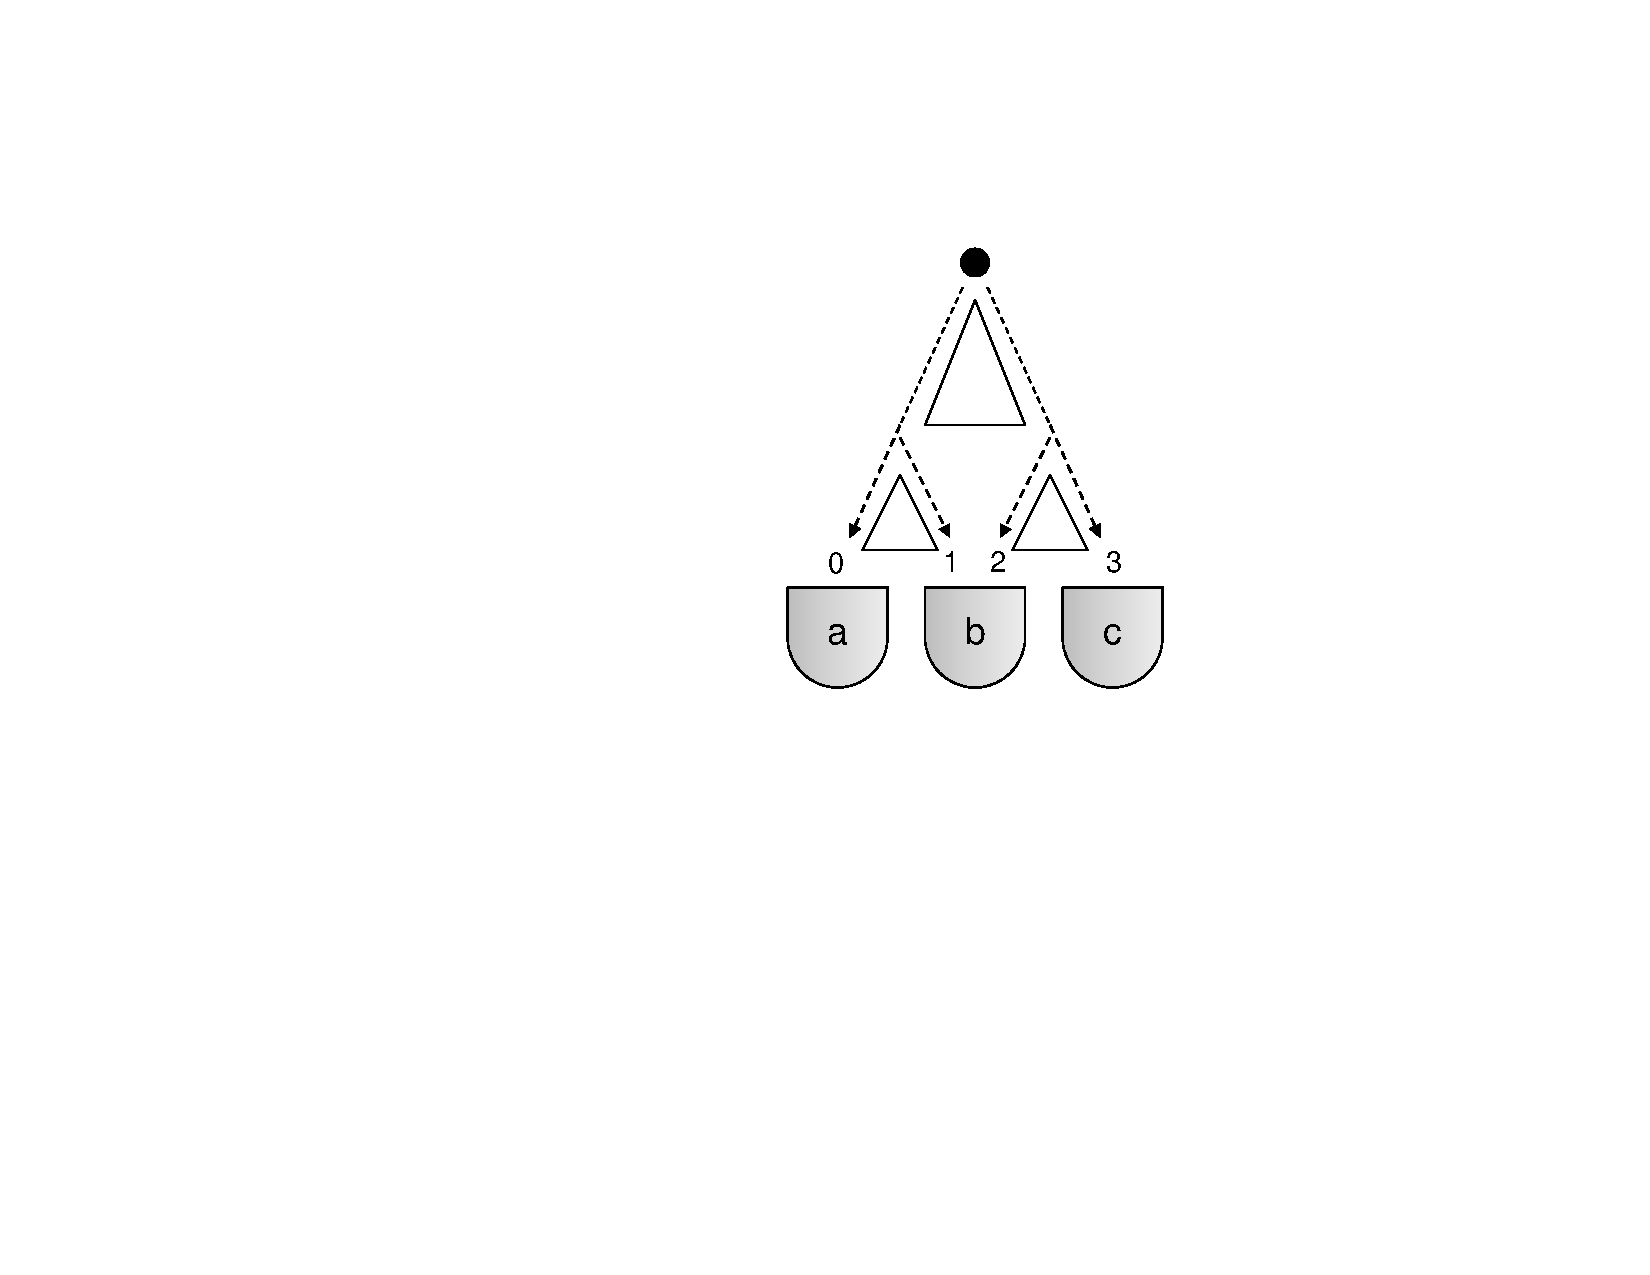
\includegraphics[scale=0.6]{figures/fig-ch6-em-marble2.pdf}
\end{center}\caption{A more complicated marble game where the released marble takes one of four possible paths.  We assume that we can only observe which cup the marble ends up in, not the specific path taken.}\label{chapter6_figure_plinko2}
\end{figure*}

To construct a statistical model of this game, we again assume that
the behavior of a marble interacting with a peg can be modeled with a
Bernoulli random variable.  Since there are three pegs, we have three
random variables with parameters $\theta=\langle p_0, p_1, p_2
\rangle$, corresponding to the probabilities that the marble will go
to the right at the top, left, and right pegs.  We further define a
random variable $X$ taking on values from $\{a,b,c\}$ indicating what
cup the marble ends in, and $Y$, taking on values from $\{0,1,2,3\}$
indicating which path was taken.  Note that the full joint
distribution $\Pr(X=x,Y=y)$ is determined by $\theta$.

How should the parameters $\theta$ be estimated?  If it were possible
to observe the paths taken by marbles as they were dropped into the
game, it would be trivial to estimate the parameters for our model
using the maximum likelihood estimator---we would simply need to count
the number of times the marble bounced left or right at each peg.  If
$N_x$ counts the number of times a marble took path $x$ in $N$ trials,
this is:

\begin{equation}
p_0 = \frac{N_2 + N_3}{N} \quad \quad p_1 = \frac{N_1}{N_0 + N_1} \quad \quad  p_2 = \frac{N_3}{N_2 + N_3}
\end{equation}

\noindent However, we wish to consider the case where the paths taken
are \emph{unobservable} (imagine an opaque sheet covering the center
of the game board), but where we can see what cup a marble ends in.
In other words, we want to consider the case where we have
\emph{partial} data.  This is exactly the problem encountered in
unsupervised learning:\ there is a statistical model describing the
relationship between two sets of variables ($X$'s and $Y$'s), and
there is data available from just one of them.  Furthermore, such
algorithms are quite useful in text processing, where latent variables
may describe latent linguistic structures of the observed variables,
such as parse trees or part-of-speech tags, or alignment structures
relating sets of observed variables (see
Section~\ref{chapter6_word_alignment}).

\subsection{MLE with Latent Variables}

Formally, we consider the problem of estimating parameters for
statistical models of the form $\Pr(X,Y;\theta)$ which describe not
only an observable variable $X$ but a latent, or hidden, variable $Y$.

In these models, since only the values of the random variable $X$ are
observable, we define our optimization criterion to be the
maximization of the \emph{marginal} likelihood, that is, summing over
all settings of the latent variable $Y$, which takes on values from
set designated $\mathcal{Y}$:\footnote{For this description, we assume
  that the variables in our model take on discrete values.  Not only
  does this simplify exposition, but discrete models are widely used
  in text processing.} Again, we assume that samples in the training
data $\textbf{x}$ are i.i.d.:
\begin{align}
\Pr(X=x) = \sum_{y \in \mathcal{Y}} \Pr(X=x,Y=y ; \theta)
\end{align}

\noindent For a vector of training observations $\textbf{x} = \langle
x_1,x_2, \ldots, x_{\ell} \rangle $, if we assume the samples are
i.i.d.:
\begin{equation}
\Pr(\textbf{x};\theta) = \prod_{j=1}^{|\textbf{x}|} \sum_{y \in \mathcal{Y}} \Pr(X=x_j,Y=y ; \theta)
\end{equation}

\noindent Thus, the maximum (marginal) likelihood estimate of the
model parameters $\theta^*$ given a vector of i.i.d. observations
$\textbf{x}$ becomes:
\begin{equation}
\theta^* = \arg \max_{\theta} \prod_{j=1}^{|\textbf{x}|} \sum_{y \in \mathcal{Y}} \Pr(X=x_j,Y=y ; \theta)
\end{equation}

\noindent Unfortunately, in many cases, this maximum cannot be
computed analytically, but the iterative hill-climbing approach of
expectation maximization can be used instead.

\subsection{Expectation Maximization}

Expectation maximization (EM) is an iterative algorithm that finds a
successive series of parameter estimates $\theta^{(0)}$,
$\theta^{(1)}$, $\ldots$ that improve the marginal likelihood of the
training data.  That is, EM guarantees:
\begin{equation}
\prod_{j=1}^{|\textbf{x}|} \sum_{y \in \mathcal{Y}} \Pr(X=x_j,Y=y ; \theta^{(i+1)}) \ge \prod_{j=1}^{|\textbf{x}|} \sum_{y \in \mathcal{Y}} \Pr(X=x_j,Y=y ; \theta^{(i)})
\end{equation}

\noindent The algorithm starts with some initial set of parameters
$\theta^{(0)}$ and then updates them using two steps:\ expectation
(E-step), which computes the posterior distribution over the latent
variables given the observable data $\textbf{x}$ and a set of
parameters $\theta^{(i)}$,\footnote{The term `expectation' is used
  since the values computed in terms of the posterior distribution
  $\Pr(\textbf{y}|\textbf{x};\theta^{(i)})$ that are required to solve
  the M-step have the form of an expectation (with respect to this
  distribution).} and maximization (M-step), which computes new
parameters $\theta^{(i+1)}$ maximizing the expected log likelihood of
the joint distribution with respect to the distribution computed in
the E-step.  The process then repeats with these new parameters.  The
algorithm terminates when the likelihood remains
unchanged.\footnote{The final solution is only guaranteed to be a
  \emph{local maximum}, but if the model is fully convex, it will also
  be the global maximum.} In more detail, the steps are as follows:

\paragraph{\textbf{E-step.}}
Compute the posterior probability of each possible hidden variable
assignments $y \in \mathcal{Y}$ for each $x \in \mathcal{X}$ and the
current parameter settings, weighted by the relative frequency with
which $x$ occurs in \textbf{x}.  Call this $q(X=x,Y=y;\theta^{(i)})$
and note that it defines a joint probability distribution over
$\mathcal{X} \times \mathcal{Y}$ in that $\sum_{(x,y) \in \mathcal{X}
  \times \mathcal{Y}} q(x,y) = 1$.
\begin{align}
q(x,y;\theta^{(i)}) & = f(x|\textbf{x}) \cdot \Pr(Y=y|X=x;\theta^{(i)}) \\
& = f(x|\textbf{x}) \cdot \frac{\Pr(x,y;\theta^{(i)})}{\sum_{y'}
  \Pr(x,y';\theta^{(i)})}
\end{align}

\paragraph{\textbf{M-step.}}
Compute new parameter settings that maximize the expected log of the
probability of the joint distribution under the $q$-distribution that
was computed in the E-step:
\begin{align}
\theta^{(i+1)} & = \arg \max_{\theta'} \mathbb{E}_{q(X=x,Y=y;\theta^{(i)})} \log \Pr(X=x,Y=y ; \theta') \\
& = \arg \max_{\theta'} \sum_{(x,y) \in \mathcal{X} \times \mathcal{Y}} q(X=x,Y=y;\theta^{(i)}) \cdot \log \Pr(X=x,Y=y ; \theta')r
\end{align}

\noindent We omit the proof that the model with parameters
$\theta^{(i+1)}$ will have equal or greater marginal likelihood on the
training data than the model with parameters $\theta^{(i)}$, but this
is provably true \cite{Jelinek_1997}.

Before continuing, we note that the effective application of
expectation maximization requires that both the E-step and the M-step
consist of tractable computations.  Specifically, summing over the
space of hidden variable assignments must not be intractable.
Depending on the independence assumptions made in the model, this may
be achieved through techniques such as dynamic programming.  However,
some models may require intractable computations.

\subsection{An EM Example}

Let's look at how to estimate the parameters from our latent variable
marble game from Section~\ref{chapter6_em_example} using EM.  We
assume training data $\textbf{x}$ consisting of $N=|\textbf{x}|$
observations of $X$ with $N_a$, $N_b$, and $N_c$ indicating the number
of marbles ending in cups $a$, $b$, and $c$.  We start with some
parameters $\theta^{(0)}=\langle p_0^{(0)}, p_1^{(0)}, p_2^{(0)}
\rangle$ that have been randomly initialized to values between 0 and
1.

\paragraph{\textbf{E-step.}}
We need to compute the distribution $q(X=x,Y=y;\theta^{(i)})$, as
defined above.  We first note that the relative frequency
$f(x|\textbf{x})$ is:
\begin{align}
f(x|\textbf{x}) = \frac{N_x}{N}
\end{align}

\noindent Next, we observe that $\Pr(Y=0|X=a)=1$ and $\Pr(Y=3|X=c)=1$
since cups $a$ and $c$ fully determine the value of the path variable
$Y$.  The posterior probability of paths 1 and 2 are only non-zero
when $X$ is $b$:
\begin{align}
\Pr(1|b;\theta^{(i)}) &= \frac{(1-p_0^{(i)}) p_1^{(i)}}{(1-p_0^{(i)}) p_1^{(i)} + p_0^{(i)} (1-p_2^{(i)})} \\
\Pr(2|b;\theta^{(i)}) &= \frac{p_0^{(i)} (1-p_2^{(i)})}{(1-p_0^{(i)}) p_1^{(i)} + p_0^{(i)} (1-p_2^{(i)})}
\end{align}

\noindent Except for the four cases just described, $\Pr(Y=y|X=x)$ is
zero for all other values of $x$ and $y$ (regardless of the value of
the parameters).

\paragraph{\textbf{M-step.}}
We now need to maximize the expectation of $\log \Pr(X,Y;\theta')$
(which will be a function in terms of the three parameter variables)
under the $q$-distribution we computed in the E step.  The non-zero
terms in the expectation are as follows:
\begin{center}
\begin{tabular}{c|c|c|c}
$x$ & $y$ & $q(X=x,Y=y;\theta^{(i)})$ & $\log \Pr(X=x,Y=y;\theta')$ \\
\hline
$a$ & 0 & $N_a/N$ & $\log (1-p'_0) + \log (1 - p'_1)$ \\
$b$ & 1 & $N_b/N \cdot \Pr(1|b;\theta^{(i)}) $ & $\log(1 - p'_0) + \log p'_1$ \\
$b$ & 2 & $N_b/N \cdot \Pr(2|b;\theta^{(i)}) $ & $\log p'_0 + \log (1-p'_2)$ \\
$c$ & 3 & $N_c/N$ & $\log p'_0 + \log p'_2$ \\
\end{tabular}
\end{center}

\noindent Multiplying across each row and adding from top to bottom
yields the expectation we wish to maximize.  Each parameter can be
optimized independently using differentiation.  The resulting optimal
values are expressed in terms of the counts in $\textbf{x}$ and
$\theta^{(i)}$:
\begin{align}
p_0 &= \frac{\Pr(2|b;\theta^{(i)}) \cdot N_b + N_c}{N} \\
p_1 &= \frac{\Pr(1|b;\theta^{(i)}) \cdot N_b}{N_a + \Pr(1|b;\theta^{(i)}) \cdot N_b} \\
p_2 &= \frac{N_c}{\Pr(2|b;\theta^{(i)}) \cdot N_b + N_c}
\end{align}

\noindent It is worth noting that the form of these expressions is
quite similar to the fully observed maximum likelihood estimate.
However, rather than depending on \emph{exact} path counts, the
statistics used are the \emph{expected} path counts, given
$\textbf{x}$ and parameters $\theta^{(i)}$.

Typically, the values computed at the end of the M-step would serve as
new parameters for another iteration of EM.  However, the example we
have presented here is quite simple and the model converges to a
global optimum after a single iteration.  For most models, EM requires
several iterations to converge, and it may not find a global optimum.
And since EM only finds a locally optimal solution, the final
parameter values depend on the values chose for $\theta^{(0)}$.

\section{Hidden Markov Models}
\label{chapter6_hmms}

To give a more substantial and useful example of models whose
parameters may be estimated using EM, we turn to hidden Markov models
(HMMs).  HMMs are models of data that are ordered \emph{sequentially}
(temporally, from left to right, etc.), such as words in a sentence,
base pairs in a gene, or letters in a word.  These simple but powerful
models have been used in applications as diverse as speech recognition
\cite{Jelinek_1997}, information extraction \cite{Seymore_1999}, gene
finding \cite{Stanke_2003}, part of speech tagging
\cite{Cutting_1992}, stock market forecasting \cite{Hassan_2005}, text
retrieval~\cite{MillerD99}, and word alignment of parallel
(translated) texts \cite{Vogel_1996} (more in
Section~\ref{chapter6_word_alignment}).

In an HMM, the data being modeled is posited to have been generated
from an underlying \emph{Markov process}, which is a stochastic
process consisting of a finite set of states where the probability of
entering a state at time $t+1$ depends only on the state of the
process at time $t$ \cite{Ross_1996}.  Alternatively, one can view a
Markov process as a probabilistic variant of a finite state machine,
where transitions are taken probabilistically.  As another point of
comparison, the PageRank algorithm considered in the previous chapter
(Section~\ref{chapter-graphs:PageRank}) can be understood as a Markov
process:\ the probability of following any link on a particular page
is independent of the path taken to reach that page.  The states of
this Markov process are, however, not directly observable (i.e., \emph{
  hidden}).  Instead, at each time step, an observable token (e.g., a
word, base pair, or letter) is emitted according to a probability
distribution conditioned on the identity of the state that the
underlying process is in.

A hidden Markov model $\mathcal{M}$ is defined as a tuple $\langle
\mathcal{S} , \mathcal{O}, \theta \rangle$.  $\mathcal{S}$ is a finite
set of states, which generate symbols from a finite observation
vocabulary $\mathcal{O}$.  Following convention, we assume that
variables $q$, $r$, and $s$ refer to states in $\mathcal{S}$, and $o$
refers to symbols in the observation vocabulary $\mathcal{O}$. This
model is parameterized by the tuple $\theta=\langle A, B, \pi \rangle$
consisting of an $|\mathcal{S}| \times |\mathcal{S}|$ matrix $A$ of
\emph{transition probabilities}, where $A_{q}(r)$ gives the
probability of transitioning from state $q$ to state $r$; an
$|\mathcal{S}| \times |\mathcal{O}|$ matrix $B$ of \emph{emission
  probabilities}, where $B_{q}(o)$ gives the probability that symbol
$o$ will be emitted from state $q$; and an $|\mathcal{S}|$-dimensional
vector $\pi$, where $\pi_q$ is the probability that the process starts
in state $q$.\footnote{This is only one possible definition of an HMM,
  but it is one that is useful for many text processing problems.  In
  alternative definitions, initial and final states may be handled
  differently, observations may be emitted during the transition
  between states, or continuous-valued observations may be emitted
  (for example, from a Gaussian distribution).}  These matrices may be
dense, but for many applications sparse parameterizations are useful.
We further stipulate that $A_{q}(r) \ge 0$, $B_q(o) \ge 0$, and $\pi_q
\ge 0$ for all $q$, $r$, and $o$, as well as that:
\begin{equation}
\sum_{r \in \mathcal{S}} A_{q}(r) = 1\ \forall q  \quad \quad \sum_{o \in \mathcal{O}} B_{q}(o) = 1\ \forall q   \quad \quad \sum_{q \in \mathcal{S}} \pi_q = 1 
\end{equation}

\noindent A sequence of observations of length $\tau$ is generated as follows:

\begin{itemize}

\item[] Step 0, let $t=1$ and select an initial state $q$ according to the distribution $\pi$.  

\item[] Step 1, an observation symbol from $\mathcal{O}$ is emitted according to the distribution $B_q$. 

\item[] Step 2, a new $q$ is drawn according to the distribution $A_q$.  

\item[] Step 3, $t$ is incremented, and if $t \le \tau$, the process repeats from Step 1.

\end{itemize}

\noindent Since all events generated by this process are conditionally
independent, the joint probability of this sequence of observations
and the state sequence used to generate it is the product of the
individual event probabilities.

Figure~\ref{chapter6_hmm_example} shows a simple example of a hidden
Markov model for part-of-speech tagging, which is the task of
assigning to each word in an input sentence its grammatical category
(one of the first steps in analyzing textual content).  States
$\mathcal{S} = \{ \textsc{det}, \textsc{adj}, \textsc{nn}, \textsc{v}
\}$ correspond to the parts of speech (determiner, adjective, noun,
and verb), and observations $\mathcal{O} = \{ \texttt{the},
\texttt{a}, \texttt{green} , \ldots \}$ are a subset of English words.
This example illustrates a key intuition behind many applications of
HMMs:\ states correspond to equivalence classes or clustering of
observations, and a single observation type may associated with
several clusters (in this example, the word \texttt{watch} can be
generated by an \textsc{nn} or \textsc{v}, since wash can either be a
noun or a verb).

\begin{figure*}
\begin{center}
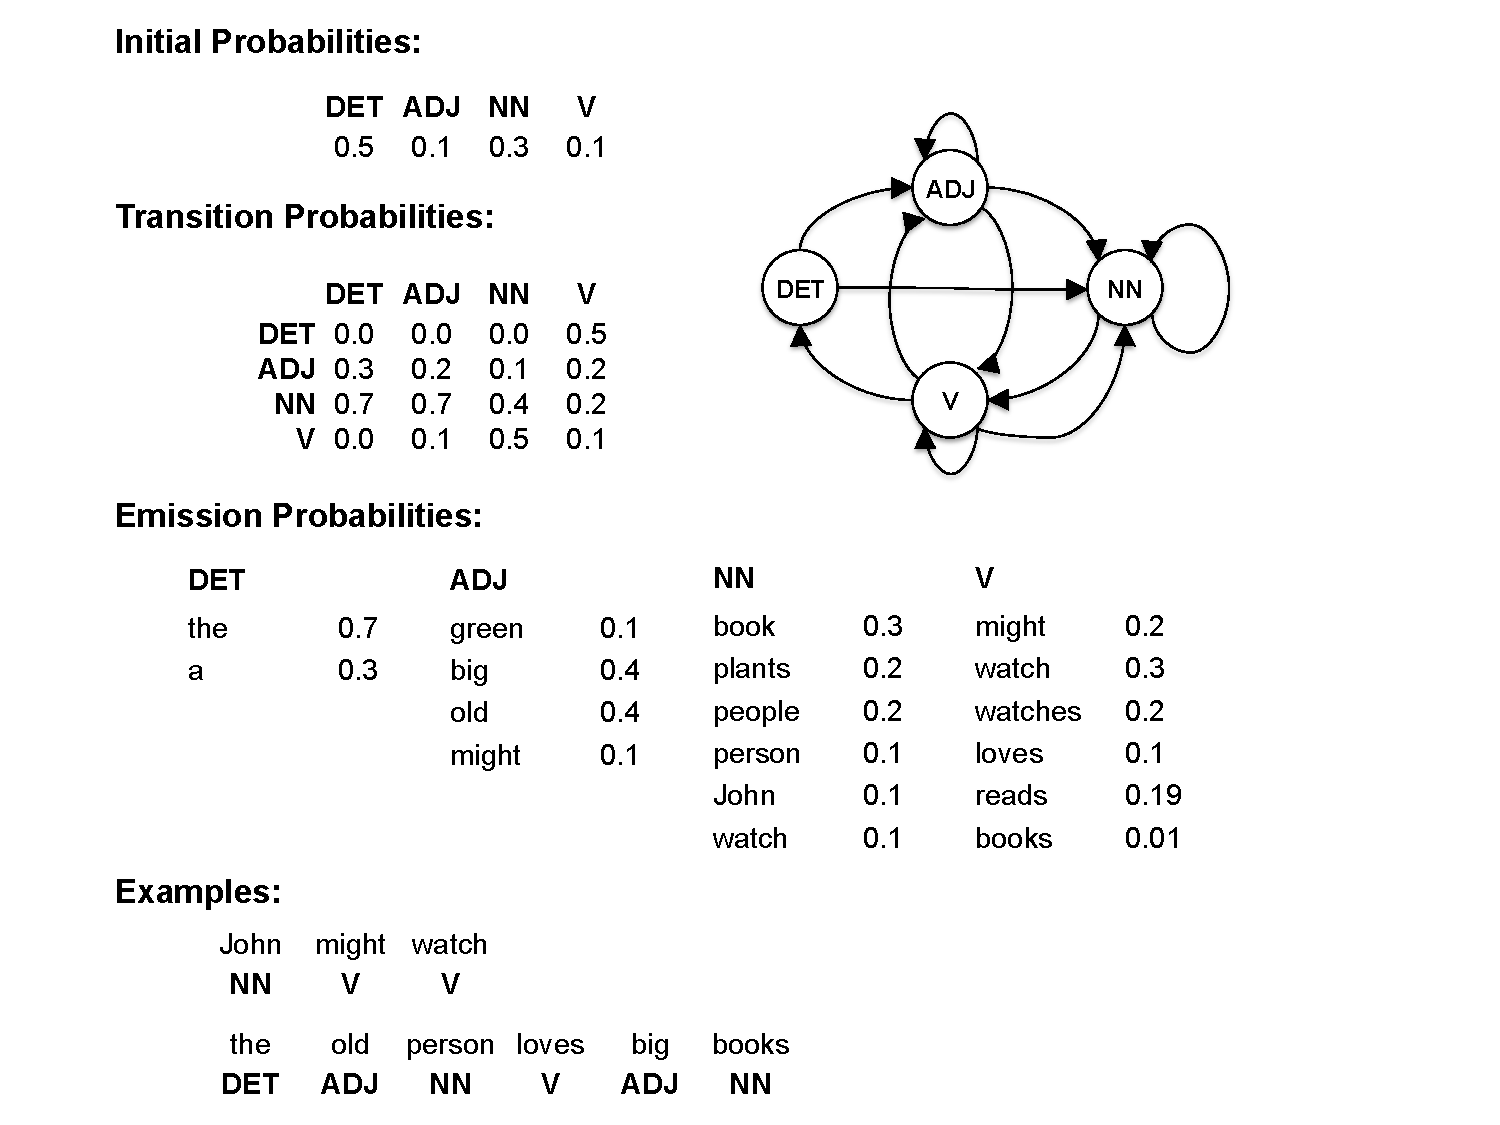
\includegraphics[scale=0.6]{figures/fig-ch6-POS-HMM.pdf}
\end{center}
\caption{An example HMM that relates part-of-speech tags to vocabulary items in an English-like language.  Possible (probability $>0$) transitions for the Markov process are shown graphically. In the example outputs, the state sequences corresponding to the emissions are written beneath the emitted symbols.}\label{chapter6_hmm_example}
\end{figure*}

\subsection{Three Questions for Hidden Markov Models}

There are three fundamental questions associated with hidden Markov
models:\footnote{The organization of this section is based in part on
  ideas from Lawrence Rabiner's HMM tutorial \cite{Rabiner_1990}.}

\begin{enumerate}
\item Given a model $\mathcal{M} = \langle \mathcal{S}, \mathcal{O}, \theta \rangle$, and an observation sequence of symbols from $\mathcal{O}$, $\textbf{x} = \langle x_1 , x_2 , \ldots , x_{\tau} \rangle$, what is the probability that $\mathcal{M}$ generated the data (summing over all possible state sequences, $\mathcal{Y}$)?
\begin{equation}
\Pr(\textbf{x}) = \sum_{\textbf{y} \in \mathcal{Y}}\Pr(\textbf{x},\textbf{y};\theta)
\end{equation}
\item Given a model $\mathcal{M} = \langle \mathcal{S}, \mathcal{O}, \theta \rangle$ and an observation sequence $\textbf{x}$, what is the most likely sequence of states that generated the data?
\begin{equation}
\textbf{y}^* = \arg \max_{\textbf{y} \in \mathcal{Y}} \Pr(\textbf{x},\textbf{y};\theta)
\end{equation}
\item Given a set of states $\mathcal{S}$, an observation vocabulary $\mathcal{O}$, and a series of $\ell$ i.i.d. observation sequences $\langle \textbf{x}_1,\textbf{x}_2,\ldots, \textbf{x}_{\ell} \rangle$, what are the parameters $\theta=\langle A, B, \pi \rangle$ that maximize the likelihood of the training data?
\begin{equation}
\theta^* = \arg \max_{\theta} \prod_{i=1}^{\ell} \sum_{\textbf{y} \in \mathcal{Y}} \Pr(\textbf{x}_i,\textbf{y};\theta)
\end{equation}
\end{enumerate}

\noindent Using our definition of an HMM, the answers to the first two
questions are in principle quite trivial to compute:\ by iterating
over all state sequences $\mathcal{Y}$, the probability that each
generated $\textbf{x}$ can be computed by looking up and multiplying
the relevant probabilities in $A$, $B$, and $\pi$, and then summing
the result or taking the maximum. And, as we hinted at in the previous
section, the third question can be answered using EM.  Unfortunately,
even with all the distributed computing power MapReduce makes
available, we will quickly run into trouble if we try to use this
na\"ive strategy since there are $|\mathcal{S}|^{\tau}$ distinct state
sequences of length $\tau$, making exhaustive enumeration
computationally intractable. Fortunately, because the underlying model
behaves exactly the same whenever it is in some state, regardless of
how it got to that state, we can use dynamic programming algorithms to
answer all of the above questions without summing over exponentially
many sequences.

\subsection{The Forward Algorithm}
\label{chapter6_forward}

Given some observation sequence, for example $\textbf{x} = \langle
\texttt{John}, \texttt{might}, \texttt{watch} \rangle$, Question 1 asks
what is the probability that this sequence was generated by an HMM
$\mathcal{M} = \langle \mathcal{S}, \mathcal{O}, \theta \rangle$.  For
the purposes of illustration, we assume that $\mathcal{M}$ is defined
as shown in Figure~\ref{chapter6_hmm_example}.

There are two ways to compute the probability of $\textbf{x}$ having
been generated by $\mathcal{M}$.  The first is to compute the sum over
the joint probability of $\textbf{x}$ and every possible labeling
$\textbf{y}' \in \{ \langle \textsc{det} , \textsc{det}, \textsc{det}
\rangle, \langle \textsc{det} , \textsc{det}, \textsc{nn} \rangle,
\langle \textsc{det} , \textsc{det}, \textsc{v} \rangle , \ldots \}$.
As indicated above this is not feasible for most sequences, since the
set of possible labels is exponential in the length of $\textbf{x}$.
The second, fortunately, is much more efficient.

We can make use of what is known as the \emph{forward algorithm} to
compute the desired probability in polynomial time.  We assume a model
$\mathcal{M} = \langle \mathcal{S}, \mathcal{O}, \theta \rangle$ as
defined above.  This algorithm works by recursively computing the
answer to a related question:\ what is the probability that the
process is in state $q$ at time $t$ and has generated $\langle x_1,
x_2, \ldots , x_t \rangle$?  Call this probability $\alpha_t(q)$.
Thus, $\alpha_t(q)$ is a two dimensional matrix (of size $|\textbf{x}|
\times |\mathcal{S}|$), called a \emph{trellis}.  It is easy to see
that the values of $\alpha_1(q)$ can be computed as the product of two
independent probabilities:\ the probability of starting in state $q$
and the probability of state $q$ generating $x_1$:
\begin{align}
\alpha_1(q) = \pi_q \cdot B_q(x_1)
\end{align}

\noindent From this, it's not hard to see that the values of
$\alpha_2(r)$ for every $r$ can be computed in terms of the
$|\mathcal{S}|$ values in $\alpha_1(\cdot)$ and the observation $x_2$:
\begin{align}
\alpha_2(r) =  B_r(x_2) \cdot \sum_{q \in \mathcal{S}} \alpha_1(q) \cdot A_q(r)
\end{align}

\noindent This works because there are $|\mathcal{S}|$ different ways
to get to state $r$ at time $t=2$:\ starting from state
$1,2,\ldots,|\mathcal{S}|$ and transitioning to state $r$.
Furthermore, because the behavior of a Markov process is determined
only by the state it is in at some time (not by how it got to that
state), $\alpha_t(r)$ can always be computed in terms of the
$|\mathcal{S}|$ values in $\alpha_{t-1}(\cdot)$ and the observation
$x_t$:
\begin{align}
\alpha_t(r) = B_r(x_t) \cdot \sum_{q \in \mathcal{S}} \alpha_{t-1}(q) \cdot A_q(r)
\end{align}

\noindent We have now shown how to compute the probability of being in
any state $q$ at any time $t$, having generated $\langle x_1, x_2,
\ldots , x_t \rangle$, with the forward algorithm.  The probability of
the full sequence is the probability of being in time $|\textbf{x}|$
and in \emph{any} state, so the answer to Question 1 can be computed
simply by summing over $\alpha$ values at time $|\textbf{x}|$ for all
states:

\begin{equation}
\Pr(\textbf{x};\theta) = \sum_{q \in \mathcal{S}} \alpha_{|\textbf{x}|}(q)
\end{equation}

\noindent In summary, there are two ways of computing the probability
that a sequence of observations $\textbf{x}$ was generated by
$\mathcal{M}$:\ exhaustive enumeration with summing and the forward
algorithm.  Figure~\ref{chapter6_fig_question1} illustrates the two
possibilities.  The upper panel shows the na\"{i}ve exhaustive
approach, enumerating all $4^3$ possible labels $\textbf{y}'$ of
$\textbf{x}$ and computing their joint probability
$\Pr(\textbf{x},\textbf{y}')$.  Summing over all $\textbf{y}'$, the
marginal probability of $\textbf{x}$ is found to be $0.00018$. The
lower panel shows the forward trellis, consisting of $4 \times 3$
cells.  Summing over the final column also yields $0.00018$, the same
result.

\begin{figure*}
\begin{center}
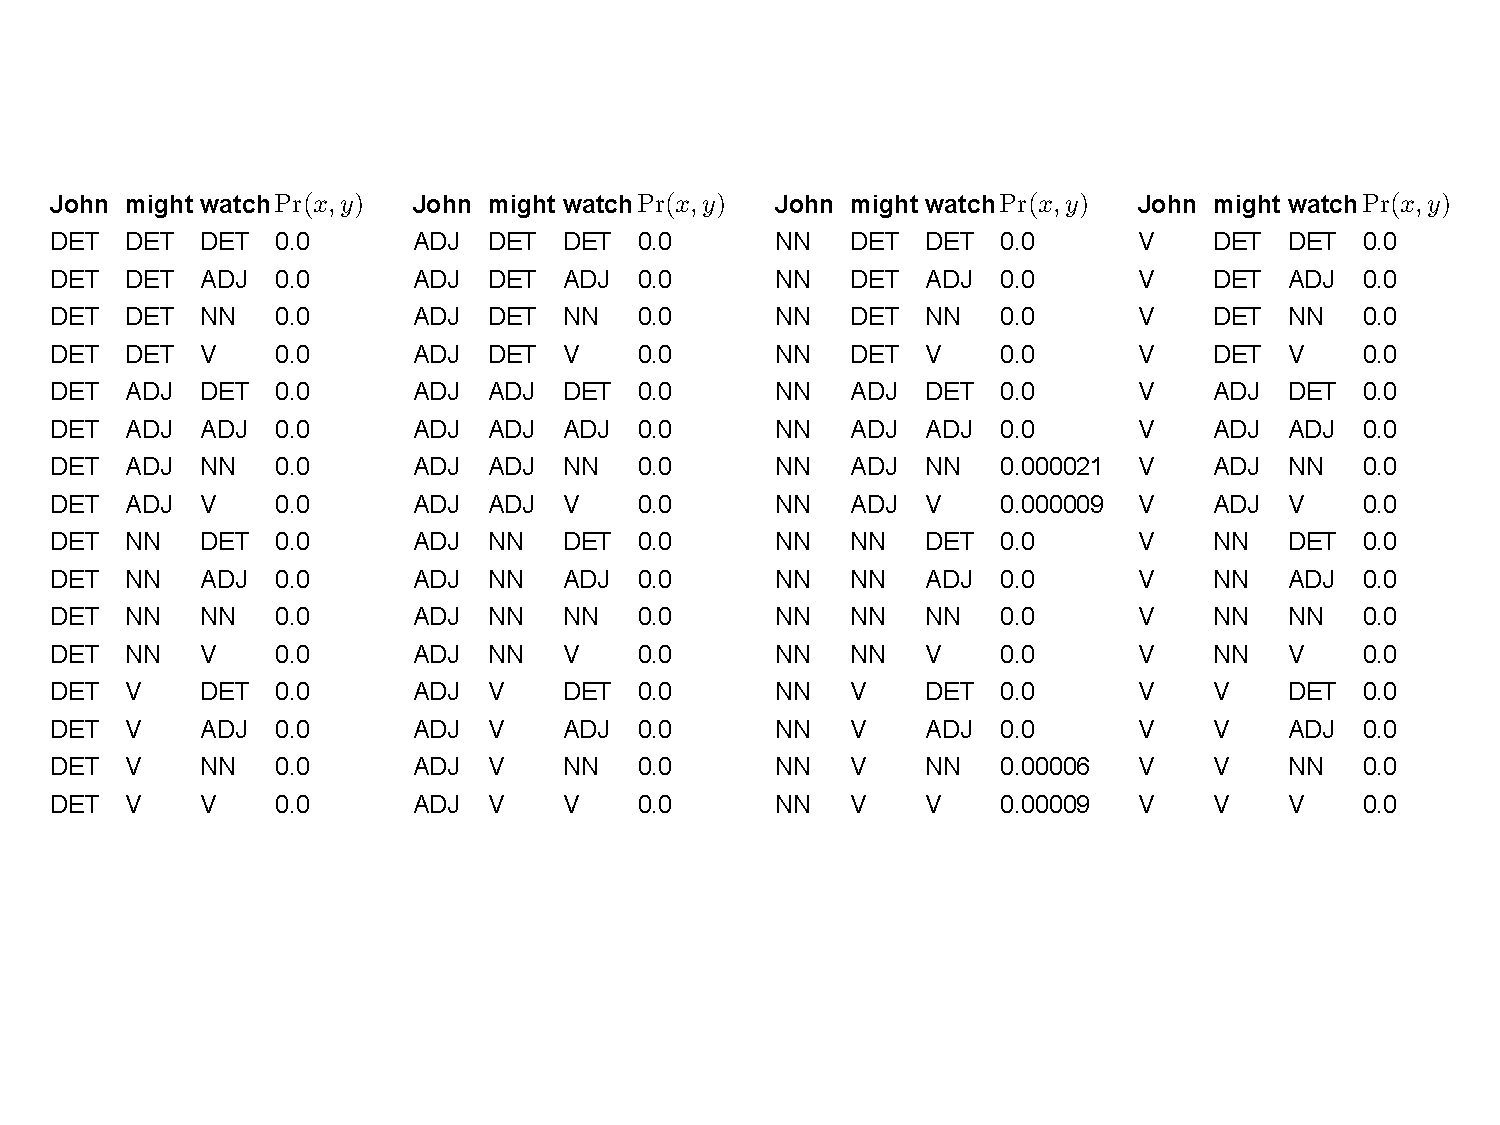
\includegraphics[scale=0.5]{figures/fig-ch6-enumerate.pdf}\\
\begin{displaymath}
\Pr(\textbf{x}) = \sum_{\textbf{y} \in \mathcal{Y}} \Pr(\textbf{x}, \textbf{y}; \theta) = 0.00018
\end{displaymath} \\

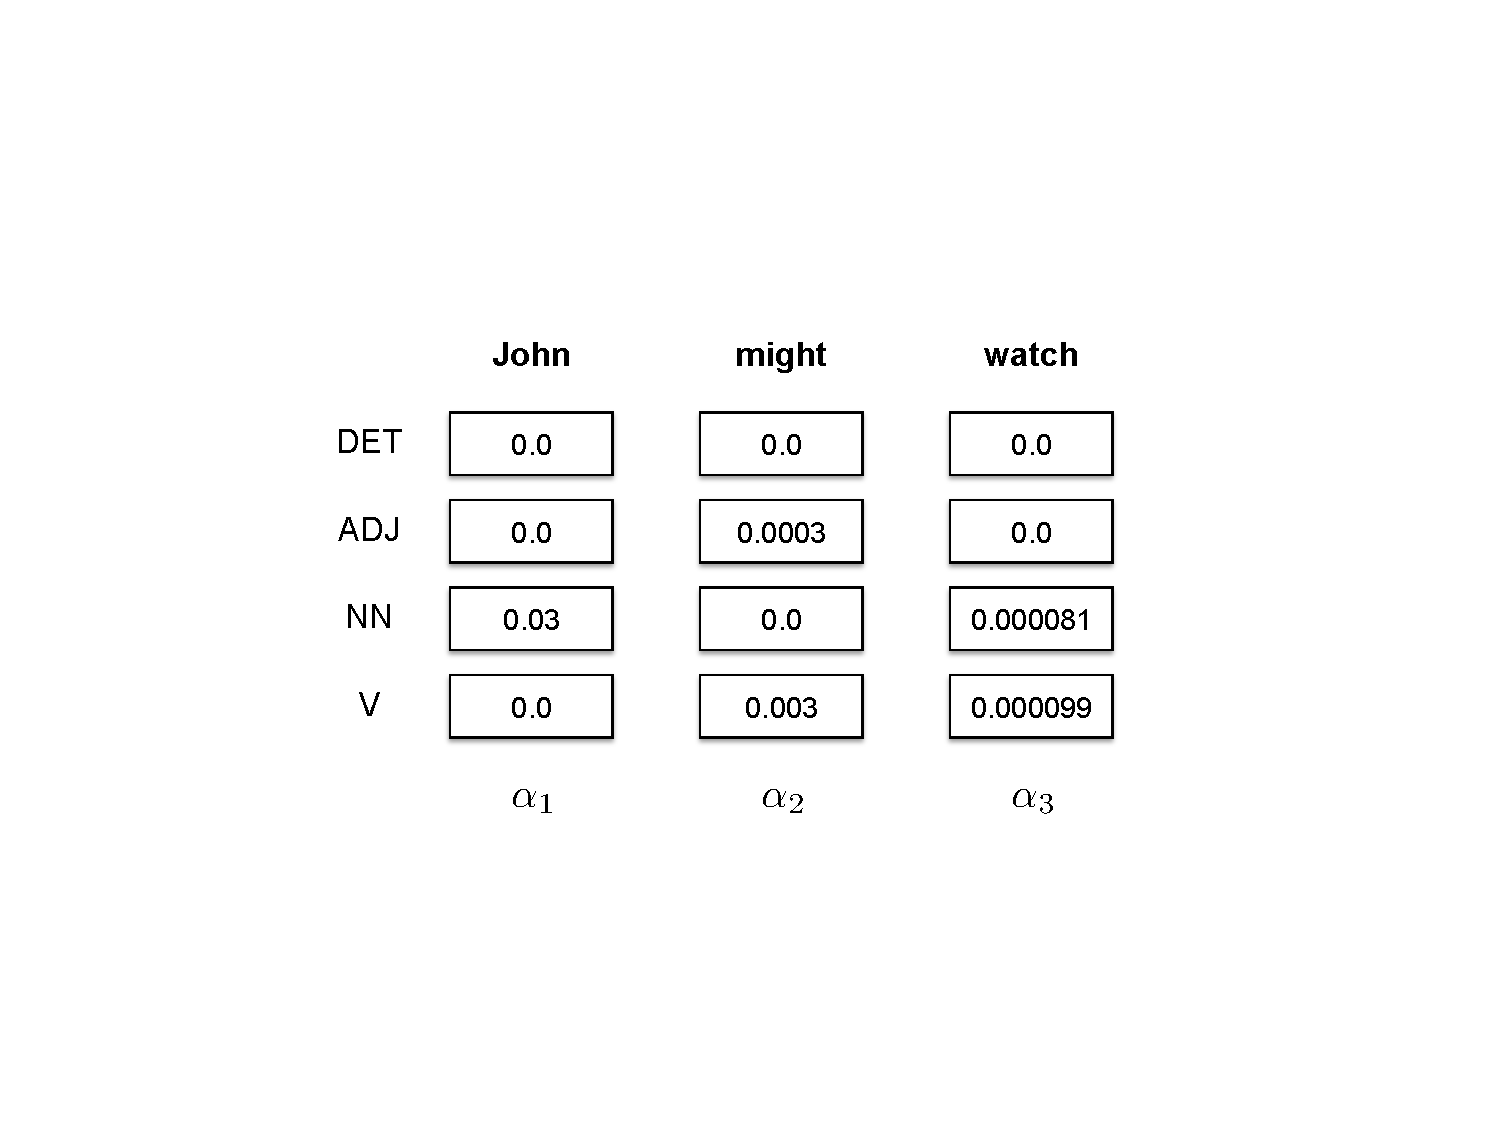
\includegraphics[scale=0.55]{figures/fig-ch6-q1new.pdf}\\
\begin{displaymath}
\Pr(\textbf{x}) = \sum_{q \in \mathcal{S}} \alpha_{3}(q) = 0.00018
\end{displaymath}
\end{center}\caption{Computing the probability of the sequence $\langle \texttt{John} , \texttt{might} , \texttt{watch} \rangle$ under the HMM given in Figure~\ref{chapter6_hmm_example} by explicitly summing over all possible sequence labels (top) and using the forward algorithm (bottom).}\label{chapter6_fig_question1}
\end{figure*}

\subsection{The Viterbi Algorithm}

Given an observation sequence $\mathbf{x}$, the second question we
might want to ask of $\mathcal{M}$ is:\ what is the most likely
sequence of states that generated the observations?  As with the
previous question, the na\"{i}ve approach to solving this problem is
to enumerate all possible labels and find the one with the highest
joint probability.  Continuing with the example observation sequence
$\textbf{x} = \langle \texttt{John} , \texttt{might} , \texttt{watch}
\rangle$, examining the chart of probabilities in the upper panel of
Figure~\ref{chapter6_fig_question1} shows that $\textbf{y}^* = \langle
\textsc{nn}, \textsc{v}, \textsc{v} \rangle$ is the most likely
sequence of states under our example HMM.

However, a more efficient answer to Question 2 can be computed using
the same intuition in the forward algorithm:\ determine the best state
sequence for a short sequence and extend this to easily compute the
best sequence for longer ones.  This is known as the \emph{Viterbi
  algorithm}.  We define $\gamma_t(q)$, the Viterbi probability, to be
the most probable sequence of states ending in state $q$ at time $t$
and generating observations $\langle x_1, x_2, \ldots , x_t \rangle$.
Since we wish to be able to reconstruct the sequence of states, we
define $bp_t(q)$, the ``backpointer'', to be the state used in this
sequence at time $t-1$.  The base case for the recursion is as follows
(the state index of $-1$ is used as a placeholder since there is no
previous best state at time $t=1$):
\begin{align}
\gamma_1(q) &= \pi_q \cdot B_q(x_1) \\
bp_1(q) & = -1
\end{align}

\noindent The recursion is similar to that of the forward algorithm,
except rather than summing over previous states, the \emph{maximum}
value of all possible trajectories into state $r$ at time $t$ is
computed.  Note that the backpointer simply records the index of the
originating state---a separate computation is not necessary.
\begin{align}
\gamma_t(r) & = \max_{q \in \mathcal{S}}  \gamma_{t-1}(q)  \cdot A_q(r) \cdot B_r(x_t)  \\
bp_t(r) & = \arg \max_{q \in \mathcal{S}} \gamma_{t-1}(q)  \cdot A_q(r) \cdot B_r(x_t)
\end{align}

\noindent To compute the best sequence of states, $\textbf{y}^*$, the
state with the highest probability path at time $|\textbf{x}|$ is
selected, and then the backpointers are followed, recursively, to
construct the rest of the sequence:
\begin{align}
y_{|\textbf{x}|}^*& = \arg \max_{q \in \mathcal{S}} \gamma_{|\textbf{x}|}(q)\\
y_{t-1}^* &= bp_t(y_t)
\end{align}

\noindent Figure~\ref{chapter6_fig_question2} illustrates a Viterbi
trellis, including backpointers that have been used to compute the
most likely state sequence.

\begin{figure*}[t]
\begin{center}
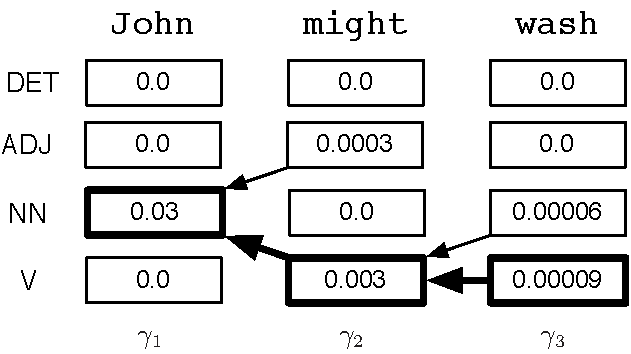
\includegraphics[scale=0.55]{figures/fig-ch6-q2.pdf}
\end{center}\caption{Computing the most likely state sequence that generated $\langle \texttt{John} , \texttt{might} , \texttt{watch} \rangle$ under the HMM given in Figure~\ref{chapter6_hmm_example} using the Viterbi algorithm.  The most likely state sequence is highlighted in bold and could be recovered programmatically by following backpointers from the maximal probability cell in the last column to the first column (thicker arrows).}\label{chapter6_fig_question2}
\end{figure*}


\subsection{Parameter Estimation for HMMs}
\label{chapter6_forward_backward}

We now turn to Question 3:\ given a set of states $\mathcal{S}$ and
observation vocabulary $\mathcal{O}$, what are the parameters
$\theta^* = \langle A,B,\pi \rangle$ that maximize the likelihood of a
set of training examples, $\langle \textbf{x}_1,\textbf{x}_2,\ldots,
\textbf{x}_{\ell} \rangle$?\footnote{Since an HMM models sequences,
  its training data consists of a collection of example sequences.}
Since our model is constructed in terms of variables whose values we
cannot observe (the state sequence) in the training data, we may train
it to optimize the marginal likelihood (summing over \emph{all} state
sequences) of $\textbf{x}$ using EM.  Deriving the EM update equations
requires only the application of the techniques presented earlier in
this chapter and some differential calculus.  However, since the
formalism is cumbersome, we will skip a detailed derivation, but
readers interested in more information can find it in the relevant
citations \cite{Jelinek_1997,Rabiner_1990}.

\begin{figure*}[t]
\begin{center}
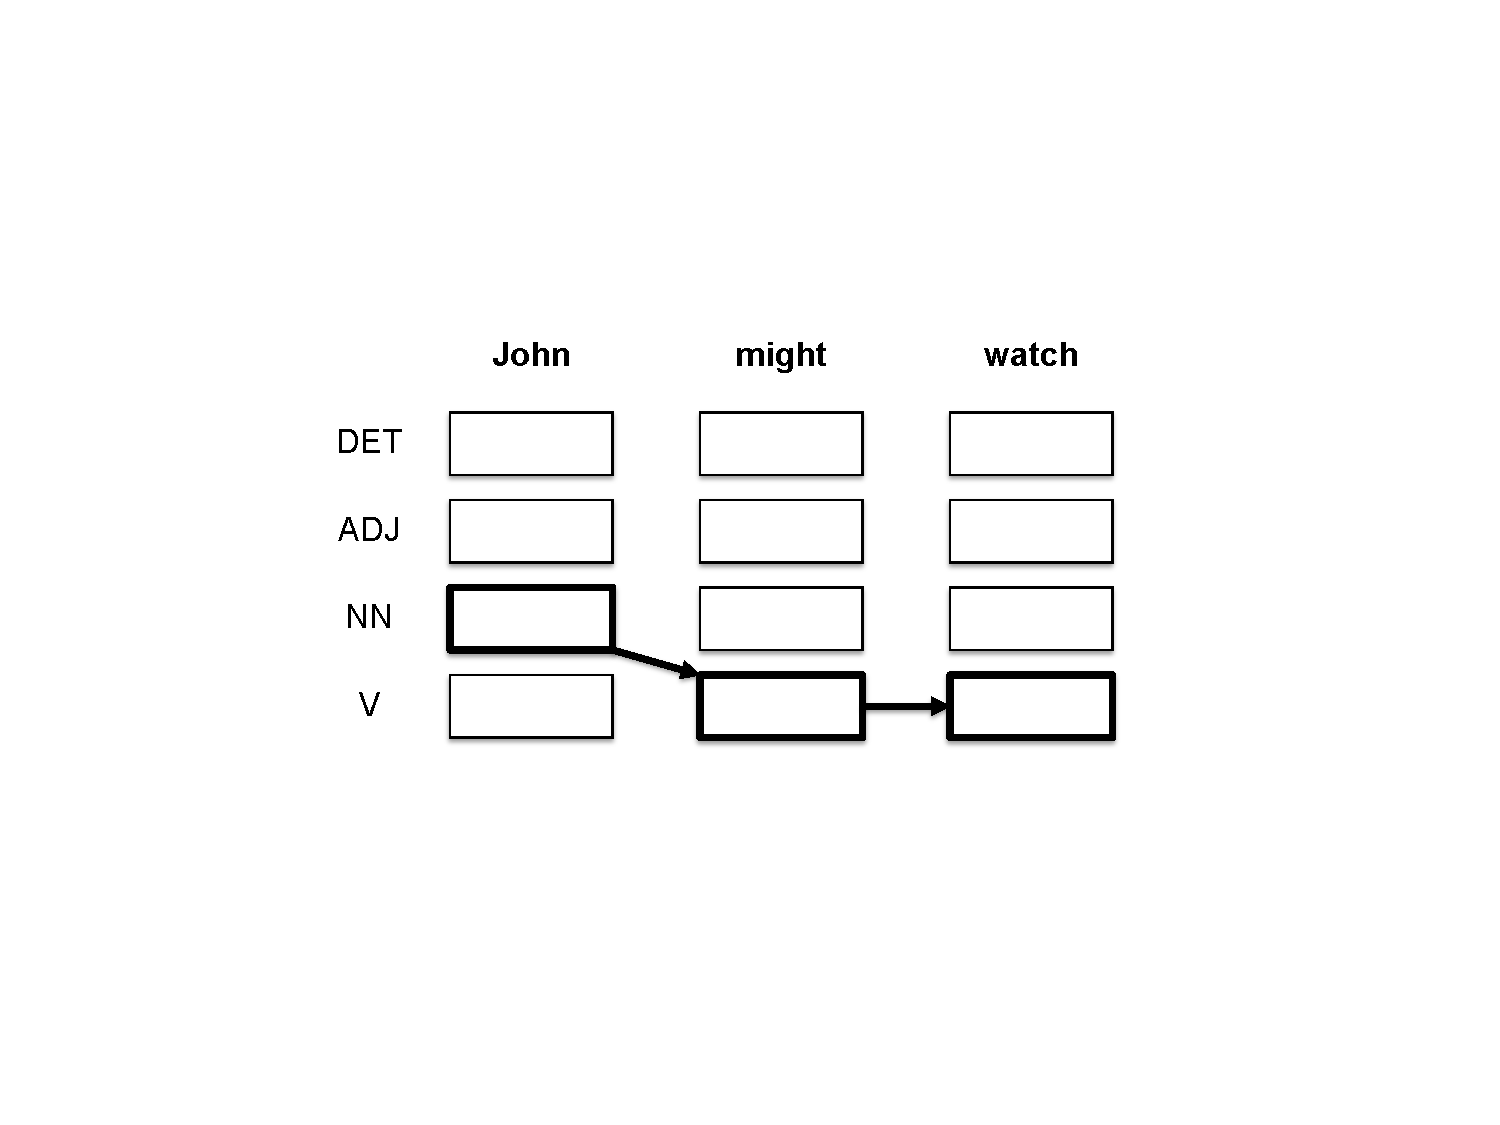
\includegraphics[scale=0.55]{figures/fig-ch6-q3a.pdf}
\end{center}\caption{A ``fully observable'' HMM training instance.  The output sequence is at the top of the figure, and the corresponding states and transitions are shown in the trellis below.}\label{chapter6_observable_hmm}
\end{figure*}

In order to make the update equations as intuitive as possible,
consider a fully observable HMM, that is, one where both the emissions
and the state sequence are observable in all $\ell$ training
instances.  In this case, a training instance can be depicted as shown
in Figure~\ref{chapter6_observable_hmm}.  When this is the case, such
as when we have a corpus of sentences in which all words have already
been tagged with their parts of speech, the maximum likelihood
estimate for the parameters can be computed in terms of the counts of
the number of times the process transitions from state $q$ to state
$r$ in all training instances, $T(q \rightarrow r)$; the number of
times that state $q$ emits symbol $o$, $O(q \uparrow o)$; and the
number of times the process starts in state $q$, $I(q)$.  In this
example, the process starts in state $\textsc{nn}$; there is one
$\textsc{nn} \rightarrow \textsc{v}$ transition and one $\textsc{v}
\rightarrow \textsc{v}$ transition.  The $\textsc{nn}$ state emits
$\texttt{John}$ in the first time step, and $\textsc{v}$ state emits
$\texttt{might}$ and $\texttt{watch}$ in the second and third time
steps, respectively. We also define $N(q)$ to be the number of times
the process enters state $q$.  The maximum likelihood estimates of the
parameters in the fully observable case are:
\begin{align}
\label{eq:chapter6_hmmopt1} 
\pi_q   &= \frac{I(q)}{\ell = \sum_{r} I(r)} \quad \\
\label{eq:chapter6_hmmopt2} 
 A_q(r) &= \frac{T(q \rightarrow r)}{N(q) = \sum_{r'} T(q \rightarrow r')} \quad\\
\label{eq:chapter6_hmmopt3} 
 B_q(o) &= \frac{O(q \uparrow o)}{N(q) = \sum_{o'} O(q \uparrow o')}
\end{align}

\noindent For example, to compute the emission parameters from state
$\textsc{nn}$, we simply need to keep track of the number of times the
process is in state $\textsc{nn}$ and what symbol it generates at each
of these times.  Transition probabilities are computed similarly:\ to
compute, for example, the distribution $A_{\textsc{det}}(\cdot)$, that
is, the probabilities of transitioning away from state $\textsc{det}$,
we count the number of times the process is in state $\textsc{det}$,
and keep track of what state the process transitioned into at the next
time step.  This counting and normalizing be accomplished using the
exact same counting and relative frequency algorithms that we
described in Section~\ref{chapter3:cond-prob}.  Thus, in the fully
observable case, parameter estimation is not a new algorithm at all,
but one we have seen before.

How should the model parameters be estimated when the state sequence
is not provided?  It turns out that the update equations have the
satisfying form where the optimal parameter values for iteration $i+1$
are expressed in terms of the \emph{expectations} of the counts
referenced in the fully observed case, according to the posterior
distribution over the latent variables given the observations
$\textbf{x}$ and the parameters $\theta^{(i)}$:
\begin{equation}
\pi_q = \frac{\mathbb{E}[I(q)]}{\ell} \quad \quad A_q(r) = \frac{\mathbb{E}[T(q \rightarrow r)]}{\mathbb{E}[N(q)]} \quad \quad B_q(o) = \frac{\mathbb{E}[O(q \uparrow o)]}{\mathbb{E}[N(q)]}
\label{chapter6_hmm_update}
\end{equation}

\noindent Because of the independence assumptions made in the HMM, the
update equations consist of $2\cdot |\mathcal{S}| + 1$ independent
optimization problems, just as was the case with the `observable' HMM.
Solving for the initial state distribution, $\pi$, is one problem;
there are $|\mathcal{S}|$ solving for the transition distributions
$A_q(\cdot)$ from each state $q$; and $|\mathcal{S}|$ solving for the
emissions distributions $B_q(\cdot)$ from each state $q$.
Furthermore, we note that the following must hold:
\begin{equation}
\mathbb{E}[N(q)] = \sum_{r \in \mathcal{S}} \mathbb{E}[T(q \rightarrow r)] = \sum_{o \in \mathcal{O}} \mathbb{E}[O(q \uparrow o)]
\end{equation}

\noindent As a result, the optimization problems (i.e.,
Equations~\ref{eq:chapter6_hmmopt1}--\ref{eq:chapter6_hmmopt3}) require completely independent
sets of statistics, which we will utilize later to facilitate
efficient parallelization in MapReduce.

How can the expectations in Equation~\ref{chapter6_hmm_update} be
understood?  In the fully observed training case, between every time
step, there is exactly one transition taken and the source and
destination states are observable.  By progressing through the Markov
chain, we can let each transition count as `1', and we can accumulate
the total number of times each kind of transition was taken (by each
kind, we simply mean the number of times that one state follows
another, for example, the number of times $\textsc{nn}$ follows
$\textsc{det}$).  These statistics can then in turn be used to compute
the MLE for an `observable' HMM, as described above.  However, when
the transition sequence is not observable (as is most often the case),
we can instead imagine that at each time step, \emph{every} possible
transition (there are $|\mathcal{S}|^2$ of them, and typically
$|\mathcal{S}|$ is quite small) is taken, with a particular
probability.  The probability used is the \emph{posterior probability}
of the transition, given the model and an observation sequence (we
describe how to compute this value below).  By summing over all the
time steps in the training data, and using this probability as the
`count' (rather than `1' as in the observable case), we compute the
\emph{expected count} of the number of times a particular transition
was taken, given the training sequence.  Furthermore, since the
training instances are statistically independent, the value of the
expectations can be computed by processing each training instance
independently and summing the results.

Similarly for the necessary emission counts (the number of times each
symbol in $\mathcal{O}$ was generated by each state in $\mathcal{S}$),
we assume that any state could have generated the observation.  We
must therefore compute the probability of being in every state at each
time point, which is then the size of the emission `count'.  By
summing over all time steps we compute the expected count of the
number of times that a particular state generated a particular symbol.
These two sets of expectations, which are written formally here, are
sufficient to execute the M-step.
\begin{align}
\label{eq:chapter6_ex1} \mathbb{E}[O(q \uparrow o)]& = \sum_{i=1}^{|\textbf{x}|} \Pr(y_i = q | \textbf{x}; \theta) \cdot \delta(x_i,o) \\
\label{eq:chapter6_ex1a} \mathbb{E}[T(q \rightarrow r)] & = \sum_{i=1}^{|\textbf{x}|-1} \Pr(y_i = q , y_{i+1} = r | \textbf{x}; \theta)
\end{align}

\paragraph{\textbf{Posterior probabilities.}}

The expectations necessary for computing the M-step in HMM training
are sums of probabilities that a particular transition is taken, given
an observation sequence, and that some state emits some observation
symbol, given an observation sequence.  These are referred to as
posterior probabilities, indicating that they are the probability of
some event whose distribution we have a prior belief about, after
addition evidence has been taken into consideration (here, the model
parameters characterize our prior beliefs, and the observation
sequence is the evidence).  Both posterior probabilities can be
computed by combining the forward probabilities, $\alpha_t(\cdot)$,
which give the probability of reaching some state at time $t$, by any
path, and generating the observations $\langle x_1, x_2, \ldots , x_t
\rangle$, with \emph{backward probabilities}, $\beta_t(\cdot)$, which
give the probability of starting in some state at time $t$ and
generating the rest of the sequence $\langle x_{t+1}, x_{t+2}, \ldots
, x_{|\textbf{x}|} \rangle$, using any sequence of states to do so.
The algorithm for computing the backward probabilities is given a bit
later.  Once the forward and backward probabilities have been
computed, the state transition posterior probabilities and the
emission posterior probabilities can be written as follows:
\begin{align}
\label{eq:chapter6_stateocprob} \Pr(y_i = q | \textbf{x}; \theta) & = \alpha_i(q) \cdot \beta_i(q) \\
\Pr(y_i = q , y_{i+1} = r | \textbf{x}; \theta) & = \alpha_i(q) \cdot A_q(r) \cdot B_r(x_{i+1}) \cdot \beta_{i+1}(r) \label{eq:chapter6_transprob}
\end{align}

\noindent Equation~\ref{eq:chapter6_stateocprob} is the probability of
being in state $q$ at time $i$, given $\textbf{x}$, and the
correctness of the expression should be clear from the definitions of
forward and backward probabilities.  The intuition for
Equation~\ref{eq:chapter6_transprob}, the probability of taking a
particular transition at a particular time, is also not
complicated:\ it is the product of four conditionally independent
probabilities:\ the probability of getting to state $q$ at time $i$
(having generated the first part of the sequence), the probability of
taking transition $q \rightarrow r$ (which is specified in the
parameters, $\theta$), the probability of generating observation
$x_{i+1}$ from state $r$ (also specified in $\theta$), and the
probability of generating the rest of the sequence, along any path.  A
visualization of the quantities used in computing this probability is
shown in Figure~\ref{chapter6_forwardbackward}.  In this illustration,
we assume an HMM with $\mathcal{S} = \{ \textsc{s}_1, \textsc{s}_2,
\textsc{s}_3 \}$ and $\mathcal{O}=\{\texttt{a}, \texttt{b}, \texttt{c}
\}$.

\begin{figure*}[t]
\begin{center}
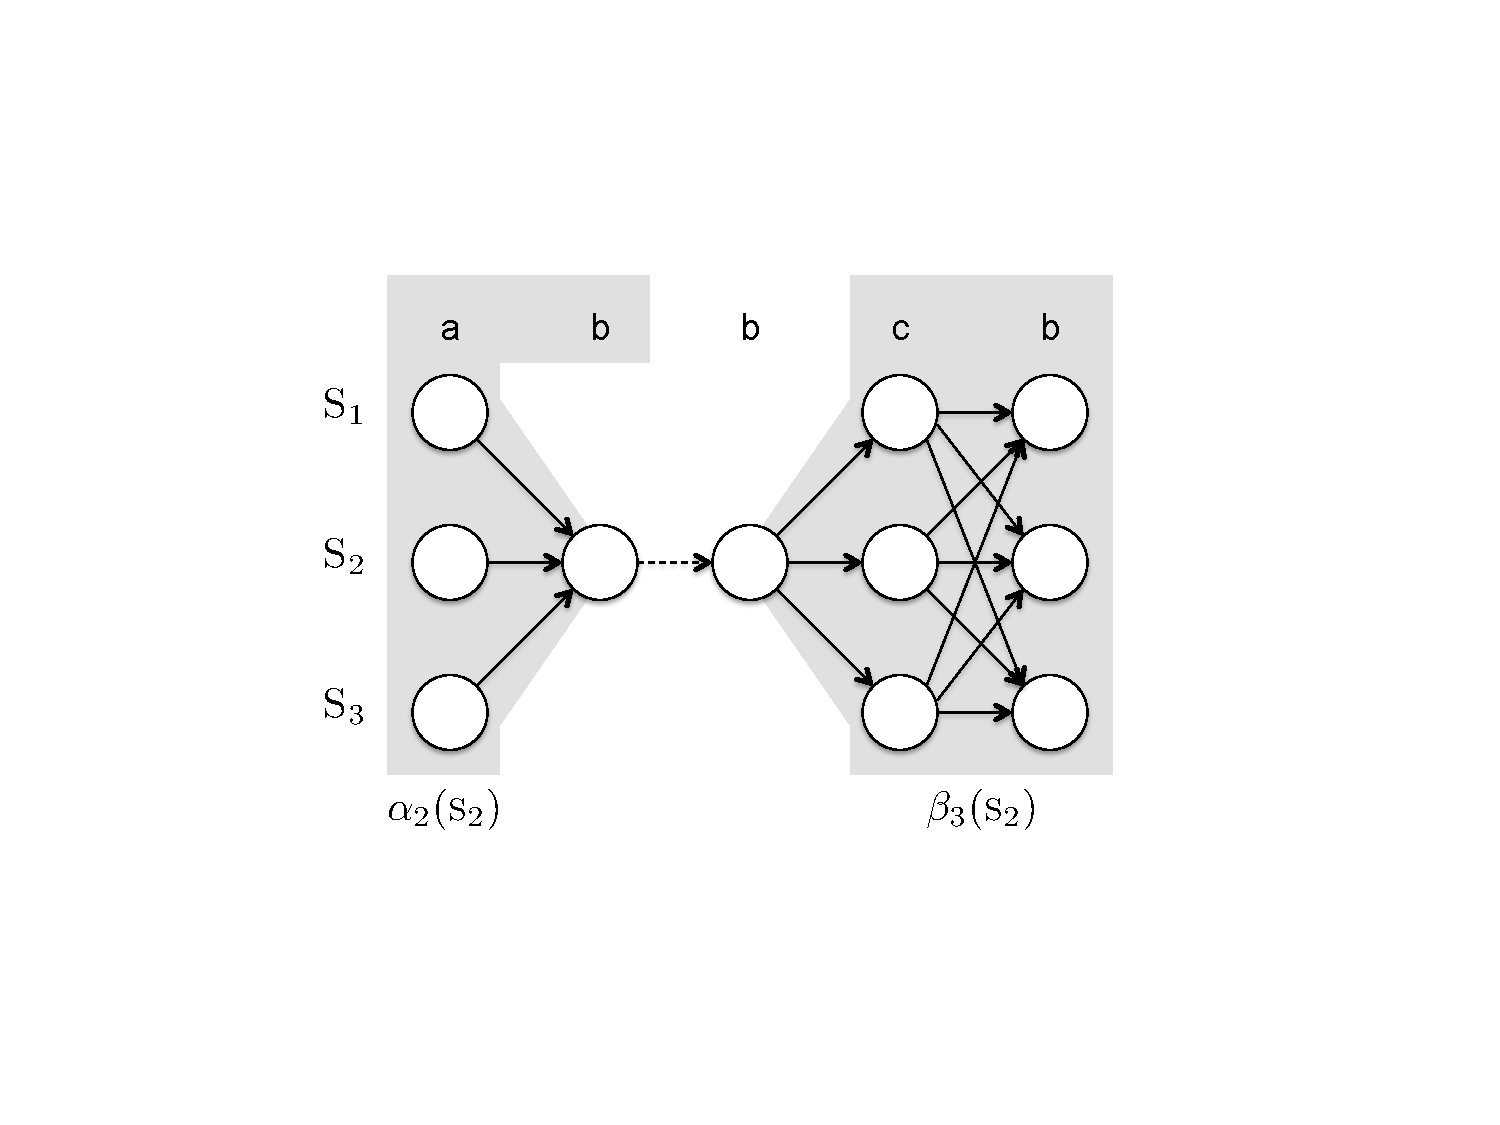
\includegraphics[scale=0.6]{figures/fig-ch6-HMM-forward-backward.pdf}
\end{center}\caption{Using forward and backward probabilities to compute the posterior probability of the dashed transition, given the observation sequence {\texttt{ a b b c b}.  The shaded area on the left corresponds to the forward probability $\alpha_{2}(\textsc{s}_2)$, and the shaded area on the right corresponds to the backward probability $\beta_3(\textsc{s}_2)$.}\label{chapter6_forwardbackward}}
\end{figure*}

\paragraph{\textbf{The backward algorithm.}}
Like the forward and Viterbi algorithms introduced above to answer
Questions 1 and 2, the backward algorithm uses dynamic programming to
incrementally compute $\beta_t(\cdot)$.  Its base case starts at time
$|\textbf{x}|$, and is defined as follows:
\label{chapter6_backward}
\begin{align}
\beta_{|\textbf{x}|}(q) = 1
\end{align}

\noindent To understand the intuition for this base case, keep in mind
that since the backward probabilities $\beta_t(\cdot)$ are the
probability of generating the remainder of the sequence \emph{after}
time $t$ (as well as being in some state), and since there is nothing
left to generate after time $|\textbf{x}|$, the probability must be 1.
The recursion is defined as follows:
\begin{align}
\beta_{t}(q) = \sum_{r \in \mathcal{S}} \beta_{t+1}(r) \cdot A_q(r) \cdot B_r(x_{t+1})
\end{align}

\noindent Unlike the forward and Viterbi algorithms, the backward
algorithm is computed from right to left and makes no reference to the
start probabilities, $\pi$.

\subsection{Forward-Backward Training:\ Summary} 

In the preceding section, we have shown how to compute all quantities
needed to find the parameter settings $\theta^{(i+1)}$ using EM
training with a hidden Markov model $\mathcal{M}=\langle
\mathcal{S},\mathcal{O}, \theta^{(i)} \rangle$.  To recap:\ each
training instance $\textbf{x}$ is processed independently, using the
parameter settings of the current iteration, $\theta^{(i)}$. For each
$\textbf{x}$ in the training data, the forward and backward
probabilities are computed using the algorithms given above (for this
reason, this training algorithm is often referred to as the
forward-backward algorithm).  The forward and backward probabilities
are in turn used to compute the expected number of times the
underlying Markov process enters into each state, the number of times
each state generates each output symbol type, and the number of times
each state transitions into each other state.  These expectations are
summed over all training instances, completing the E-step.  The M-step
involves normalizing the expected counts computed in the E-step using
the calculations in Equation~\ref{chapter6_hmm_update}, which yields
$\theta^{(i+1)}$.  The process then repeats from the E-step using the
new parameters.  The number of iterations required for convergence
depends on the quality of the initial parameters, and the complexity
of the model.  For some applications, only a handful of iterations are
necessary, whereas for others, hundreds may be required.

Finally, a few practical considerations:\ HMMs have a non-convex
likelihood surface (meaning that it has the equivalent of many hills
and valleys in the number of dimensions corresponding to the number of
parameters in the model).  As a result, EM training is only guaranteed
to find a local maximum, and the quality of the learned model may vary
considerably, depending on the initial parameters that are used.
Strategies for optimal selection of initial parameters depend on the
phenomena being modeled.  Additionally, if some parameter is assigned
a probability of 0 (either as an initial value or during one of the
M-step parameter updates), EM will never change this in future
iterations.  This can be useful, since it provides a way of
constraining the structures of the Markov model; however, one must be
aware of this behavior.

Another pitfall to avoid when implementing HMMs is arithmetic
underflow.  HMMs typically define a massive number of sequences, and
so the probability of any one of them is often vanishingly small---so
small that they often underflow standard floating point
representations.  A very common solution to this problem is to
represent probabilities using their logarithms.  Note that expected
counts do not typically have this problem and can be represented using
normal floating point numbers.  See
Section~\ref{chapter-graphs:issues} for additional discussion on
working with log probabilities.

\section{EM in MapReduce}
\label{chapter6_mapreduce}

Expectation maximization algorithms fit quite naturally into the
MapReduce programming model.  Although the model being optimized
determines the details of the required computations, MapReduce
implementations of EM algorithms share a number of characteristics:

\begin{itemize}

\item Each iteration of EM is one MapReduce job.

\item A controlling process (i.e., driver program) spawns the
  MapReduce jobs, keeps track of the number of iterations and
  convergence criteria.

\item Model parameters $\theta^{(i)}$, which are static for the
  duration of the MapReduce job, are loaded by each mapper from HDFS
  or other data provider (e.g., a distributed key-value store).

\item Mappers map over independent training instances, computing
  partial latent variable posteriors (or summary statistics, such as
  expected counts).

\item Reducers sum together the required training statistics
  \emph{and} solve one or more of the M-step optimization problems.

\item Combiners, which sum together the training statistics, are often
  quite effective at reducing the amount of data that must be written
  to disk.

\end{itemize}

\noindent The degree of parallelization that can be attained depends
on the statistical independence assumed in the model and in the
derived quantities required to solve the optimization problems in the
M-step.  Since parameters are estimated from a collection of samples
that are assumed to be i.i.d., the E-step can generally be
parallelized effectively since every training instance can be
processed independently of the others.  In the limit, in fact, each
independent training instance could be processed by a separate
mapper!\footnote{Although the wisdom of doing this is questionable,
  given that the startup costs associated with individual map tasks in
  Hadoop may be considerable.}

Reducers, however, must aggregate the statistics necessary to solve
the optimization problems as required by the model.  The degree to
which these may be solved independently depends on the structure of
the model, and this constrains the number of reducers that may be
used.  Fortunately, many common models (such as HMMs) require solving
several independent optimization problems in the M-step.  In this
situation, a number of reducers may be run in parallel.  Still, it is
possible that in the worst case, the M-step optimization problem will
not decompose into independent subproblems, making it necessary to use
a single reducer.

\subsection{HMM Training in MapReduce}

As we would expect, the training of hidden Markov models parallelizes
well in MapReduce.  The process can be summarized as follows:\ in each
iteration, mappers process training instances, emitting expected event
counts computed using the forward-backward algorithm introduced in
Section~\ref{chapter6_forward_backward}.  Reducers aggregate the
expected counts, completing the E-step, and then generate parameter
estimates for the next iteration using the updates given in
Equation~\ref{chapter6_hmm_update}.

This parallelization strategy is effective for several reasons.
First, the majority of the computational effort in HMM training is the
running of the forward and backward algorithms.  Since there is no
limit on the number of mappers that may be run, the full computational
resources of a cluster may be brought to bear to solve this problem.
Second, since the M-step of an HMM training iteration with
$|\mathcal{S}|$ states in the model consists of $2\cdot |\mathcal{S}|
+ 1$ independent optimization problems that require non-overlapping
sets of statistics, this may be exploited with as many as $2\cdot
|\mathcal{S}| + 1$ reducers running in parallel.  While the
optimization problem is computationally trivial, being able to reduce
in parallel helps avoid the data bottleneck that would limit
performance if only a single reducer is used.

The quantities that are required to solve the M-step optimization
problem are quite similar to the relative frequency estimation example
discussed in Section~\ref{chapter3:cond-prob}; however, rather than
counts of observed events, we aggregate \emph{expected} counts of
events.  As a result of the similarity, we can employ the \emph{
  stripes} representation for aggregating sets of related values, as
described in Section~\ref{chapter3:pairs-and-stripes}.  A \emph{pairs}
approach that requires less memory at the cost of slower performance
is also feasible.

\begin{figure*}[t]
\algrenewcommand\algorithmicfunction{\textbf{class}}
\algrenewcommand\algorithmicprocedure{\textbf{method}}
  \begin{algorithmic}[1]
    \Function{Mapper}{}
    \Procedure{Initialize}{$\textrm{integer \emph{iteration}}$}
    \State $\langle \mathcal{S}, \mathcal{O} \rangle \gets \textsc{ReadModel}$
    \State $\theta \gets \langle A , B , \pi \rangle \gets \textsc{ReadModelParams}(iteration)$
    \EndProcedure
    \Procedure{Map}{$\textrm{sample }id, \textrm{sequence }\textbf{x}$}
        \State $\alpha \gets \textsc{Forward}(\textbf{x},\theta)$ \Comment{\emph{cf.} Section~\ref{chapter6_forward}}
        \State $\beta \gets \textsc{Backward}(\textbf{x},\theta)$ \Comment{\emph{cf.} Section~\ref{chapter6_backward}}
        \State $I \gets \textrm{new }\textsc{AssociativeArray}$ \Comment{Initial state expectations}
        \ForAll{$q \in \mathcal{S}$}   \Comment{Loop over states}
          \State $I\{q\} \gets \alpha_1(q) \cdot \beta_1(q)$
        \EndFor
        
        \State $O \gets \textrm{new }\textsc{AssociativeArray}\textrm{ of }\textsc{AssociativeArray}$ \Comment{Emissions}
        \For{$t = 1$ to $|\textbf{x}|$}  \Comment{Loop over observations}
        \ForAll{$q \in \mathcal{S}$}   \Comment{Loop over states}
           \State $O\{q\}\{x_t\} \gets O\{q\}\{x_t\} + \alpha_t(q) \cdot \beta_t(q)$
        \EndFor
           \State $t \leftarrow t + 1$
        \EndFor

        \State $T \gets \textrm{new }\textsc{AssociativeArray}\textrm{ of }\textsc{AssociativeArray}$
        \State \Comment{Transitions}
        \For{$t = 1$ to $|\textbf{x}|-1$}  \Comment{Loop over observations}
        \ForAll{$q \in \mathcal{S}$}   \Comment{Loop over states}
        \ForAll{$r \in \mathcal{S}$}   \Comment{Loop over states}
           \State $T\{q\}\{r\} \gets T\{q\}\{r\} + \alpha_t(q) \cdot A_q(r) \cdot B_r(x_{t+1}) \cdot \beta_{t+1}(r)$
        \EndFor
        \EndFor
        \State $t \leftarrow t + 1$
        \EndFor

        \State $\textsc{Emit}(\textrm{string `\emph{initial}'}, \textrm{stripe }I)$
        \ForAll{$q \in \mathcal{S}$}   \Comment{Loop over states}
           \State $\textsc{Emit}(\textrm{string `\emph{emit from }'}+q, \textrm{stripe }O\{q\})$
           \State $\textsc{Emit}(\textrm{string `\emph{transit from }'}+q, \textrm{stripe }T\{q\})$
        \EndFor

    \EndProcedure
    \EndFunction
  \end{algorithmic}
  \caption{Mapper pseudo-code for training hidden Markov models using EM.  The mappers map over training instances (i.e., sequences of observations $\textbf{x}_i$) and generate the expected counts of initial states, emissions, and transitions taken to generate the sequence.}
\label{figure:chapter6:mr_hmm_mapper}
\end{figure*}

\begin{figure*}[t]
\algrenewcommand\algorithmicfunction{\textbf{class}}
\algrenewcommand\algorithmicprocedure{\textbf{method}}
  \begin{algorithmic}[1]
    \Function{Combiner}{}
    \Procedure{Combine}{$\textrm{string }t, \textrm{stripes }[ C_1, C_2, \ldots ]$}
        \State $C_f \gets \textrm{new }\textsc{AssociativeArray}$
    \ForAll{$ \textrm{stripe }C \in \textrm{stripes }[ C_1, C_2, \ldots ]$}
        \State $\textsc{Sum}(C_f, C)$
    \EndFor
     \State $\textsc{Emit}(\textrm{string }t, \textrm{stripe }C_f)$
    \EndProcedure
    \EndFunction
  \end{algorithmic}
  \begin{algorithmic}[1]
    \Function{Reducer}{}
    \Procedure{Reduce}{$\textrm{string }t, \textrm{stripes }[ C_1, C_2, \ldots ]$}
        \State $C_f \gets \textrm{new }\textsc{AssociativeArray}$
    \ForAll{$ \textrm{stripe }C \in \textrm{stripes }[ C_1, C_2, \ldots ]$}
        \State $\textsc{Sum}(C_f, C)$
    \EndFor
    \State $z \gets 0$
    \ForAll{$\langle k, v \rangle \in C_f$}
	\State $z \gets z + v$
    \EndFor
    \State $P_f \gets \textrm{new }\textsc{AssociativeArray}$\Comment{Final parameters vector}
    \ForAll{$\langle k, v \rangle \in C_f$}
	\State $P_f\{k\} \gets v / z$    
    \EndFor
     \State $\textsc{Emit}(\textrm{string }t, \textrm{stripe }P_f)$
    \EndProcedure
    \EndFunction
  \end{algorithmic}
  \caption{Combiner and reducer pseudo-code for training hidden Markov models using EM. The HMMs considered in this book are fully parameterized by multinomial distributions, so reducers do not require special logic to handle different types of model parameters (since they are all of the same type).}
\label{figure:chapter6:mr_hmm_reducer}
\end{figure*}

\paragraph{\textbf{HMM training mapper.}}
The pseudo-code for the HMM training mapper is given in
Figure~\ref{figure:chapter6:mr_hmm_mapper}.  The input consists of
key-value pairs with a unique id as the key and a training instance
(e.g., a sentence) as the value.  For each training instance, $2n+1$
stripes are emitted with unique keys, and every training instance
emits the same set of keys.  Each unique key corresponds to one of the
independent optimization problems that will be solved in the M-step.
The outputs are:

\begin{enumerate}
\item the probabilities that the unobserved Markov process begins in
  each state $q$, with a unique key designating that the values are
  initial state counts;

\item the expected number of times that state $q$ generated each
  emission symbol $o$ (the set of emission symbols included will be
  just those found in each training instance $\textbf{x}$), with a key
  indicating that the associated value is a set of \emph{emission}
  counts from state $q$; and

\item the expected number of times state $q$ transitions to each state
  $r$, with a key indicating that the associated value is a set of
  \emph{transition} counts from state $q$.

\end{enumerate}

\paragraph{\textbf{HMM training reducer.}}
The reducer for one iteration of HMM training, shown together with an
optional combiner in Figure~\ref{figure:chapter6:mr_hmm_reducer},
aggregates the count collections associated with each key by summing
them.  When the values for each key have been completely aggregated,
the associative array contains all of the statistics necessary to
compute a subset of the parameters for the next EM iteration.  The
optimal parameter settings for the following iteration are computed
simply by computing the relative frequency of each event with respect
to its expected count at the current iteration.  The new computed
parameters are emitted from the reducer and written to HDFS.  Note
that they will be spread across $2\cdot | \mathcal{S} |+1$ keys,
representing initial state probabilities $\pi$, transition
probabilities $A_q$ for each state $q$, and emission probabilities
$B_q$ for each state $q$.


\section{Case Study:\ Word Alignment for Statistical Machine Translation}
\label{chapter6_word_alignment}

To illustrate the real-world benefits of expectation maximization
algorithms using MapReduce, we turn to the problem of word alignment,
which is an important task in statistical machine translation that is
typically solved using models whose parameters are learned with EM.

We begin by giving a brief introduction to statistical machine
translation and the phrase-based translation approach; for a more
comprehensive introduction, refer to \cite{Koehn_2009,Lopez_2008}.
Fully-automated translation has been studied since the earliest days
of electronic computers.  After successes with code-breaking during
World War II, there was considerable optimism that translation of
human languages would be another soluble problem. In the early years,
work on translation was dominated by manual attempts to encode
linguistic knowledge into computers---another instance of the
`rule-based' approach we described in the introduction to this
chapter.  These early attempts failed to live up to the admittedly
optimistic expectations.  For a number of years, the idea of fully
automated translation was viewed with skepticism.  Not only was
constructing a translation system labor intensive, but translation
pairs had to be developed independently, meaning that improvements in
a Russian-English translation system could not, for the most part, be
leveraged to improve a French-English system.

After languishing for a number of years, the field was reinvigorated
in the late 1980s when researchers at IBM pioneered the development of
\emph{statistical machine translation} (SMT), which took a data-driven
approach to solving the problem of machine translation, attempting to
improve both the quality of translation while reducing the cost of
developing systems \cite{Brown_1993}.  The core idea of SMT is to
equip the computer to \emph{learn} how to translate, using example
translations which are produced for other purposes, and modeling the
process as a statistical process with some parameters $\theta$
relating strings in a source language (typically denoted as
$\textbf{f}$) to strings in a target language (typically denoted as
$\textbf{e}$):
\begin{align}
\textbf{e}^* = \arg \max_{\textbf{e}} \Pr(\textbf{e} | \textbf{f} ; \theta)
\end{align}

With the statistical approach, translation systems can be developed
cheaply and quickly for any language pair, as long as there is
sufficient training data available.  Furthermore, improvements in
learning algorithms and statistical modeling can yield benefits in
many translation pairs at once, rather than being specific to
individual language pairs.  Thus, SMT, like many other topics we are
considering in this book, is an attempt to leverage the vast
quantities of textual data that is available to solve problems that
would otherwise require considerable manual effort to encode
specialized knowledge. Since the advent of statistical approaches to
translation, the field has grown tremendously and numerous statistical
models of translation have been developed, with many incorporating
quite specialized knowledge about the behavior of natural language as
biases in their learning algorithms.

\subsection{Statistical Phrase-Based Translation}

One approach to statistical translation that is simple yet powerful is
called \emph{phrase-based translation} \cite{Koehn_2003}.  We provide
a rough outline of the process since it is representative of most
state-of-the-art statistical translation systems, such as the one used
inside Google Translate.\footnote{\texttt{http://translate.google.com}}
Phrase-based translation works by learning how strings of words,
called \emph{phrases}, translate between languages.\footnote{Phrases
  are simply sequences of words; they are not required to correspond
  to the definition of a phrase in any linguistic theory.}  Example
phrase pairs for Spanish-English translation might include:

\begin{quote}
$\langle \textrm{\emph{los estudiantes}}, \textrm{\emph{the students}}\rangle$,
$\langle \textrm{\emph{los estudiantes}}, \textrm{\emph{some
    students}}\rangle$, and $\langle \textrm{\emph{soy}},
\textrm{\emph{i am}} \rangle$.
\end{quote}

\noindent From a few hundred thousand sentences
of example translations, many millions of such phrase pairs may be
automatically learned.

The starting point is typically a parallel corpus (also called \emph{
  bitext}), which contains \emph{pairs} of sentences in two languages
that are translations of each other. Parallel corpora are frequently
generated as the byproduct of an organization's effort to disseminate
information in multiple languages, for example, proceedings of the
Canadian Parliament in French and English, and text generated by the
United Nations in many different languages.  The parallel corpus is
then annotated with \emph{word alignments}, which indicate which words
in one language correspond to words in the other.  By using these word
alignments as a skeleton, phrases can be extracted from the sentence
that is likely to preserve the meaning relationships represented by
the word alignment.  While an explanation of the process is not
necessary here, we mention it as a motivation for learning word
alignments, which we show below how to compute with EM.  After phrase
extraction, each phrase pair is associated with a number of scores
which, taken together, are used to compute the phrase translation
probability, a conditional probability that reflects how likely the
source phrase translates into the target phrase.  We briefly note that
although EM could be utilized to learn the phrase translation
probabilities, this is not typically done in practice since the
maximum likelihood solution turns out to be quite bad for this
problem.  The collection of phrase pairs and their scores are referred
to as the \emph{translation model}.  In addition to the translation
model, phrase-based translation depends on a \emph{language model},
which gives the probability of a string in the target language.  The
translation model attempts to preserve the meaning of the source
language during the translation process, while the language model
ensures that the output is fluent and grammatical in the target
language.  The phrase-based translation process is summarized in
Figure~\ref{chapter6_figure_mtarch}.

\begin{figure*}[p]
\begin{center}
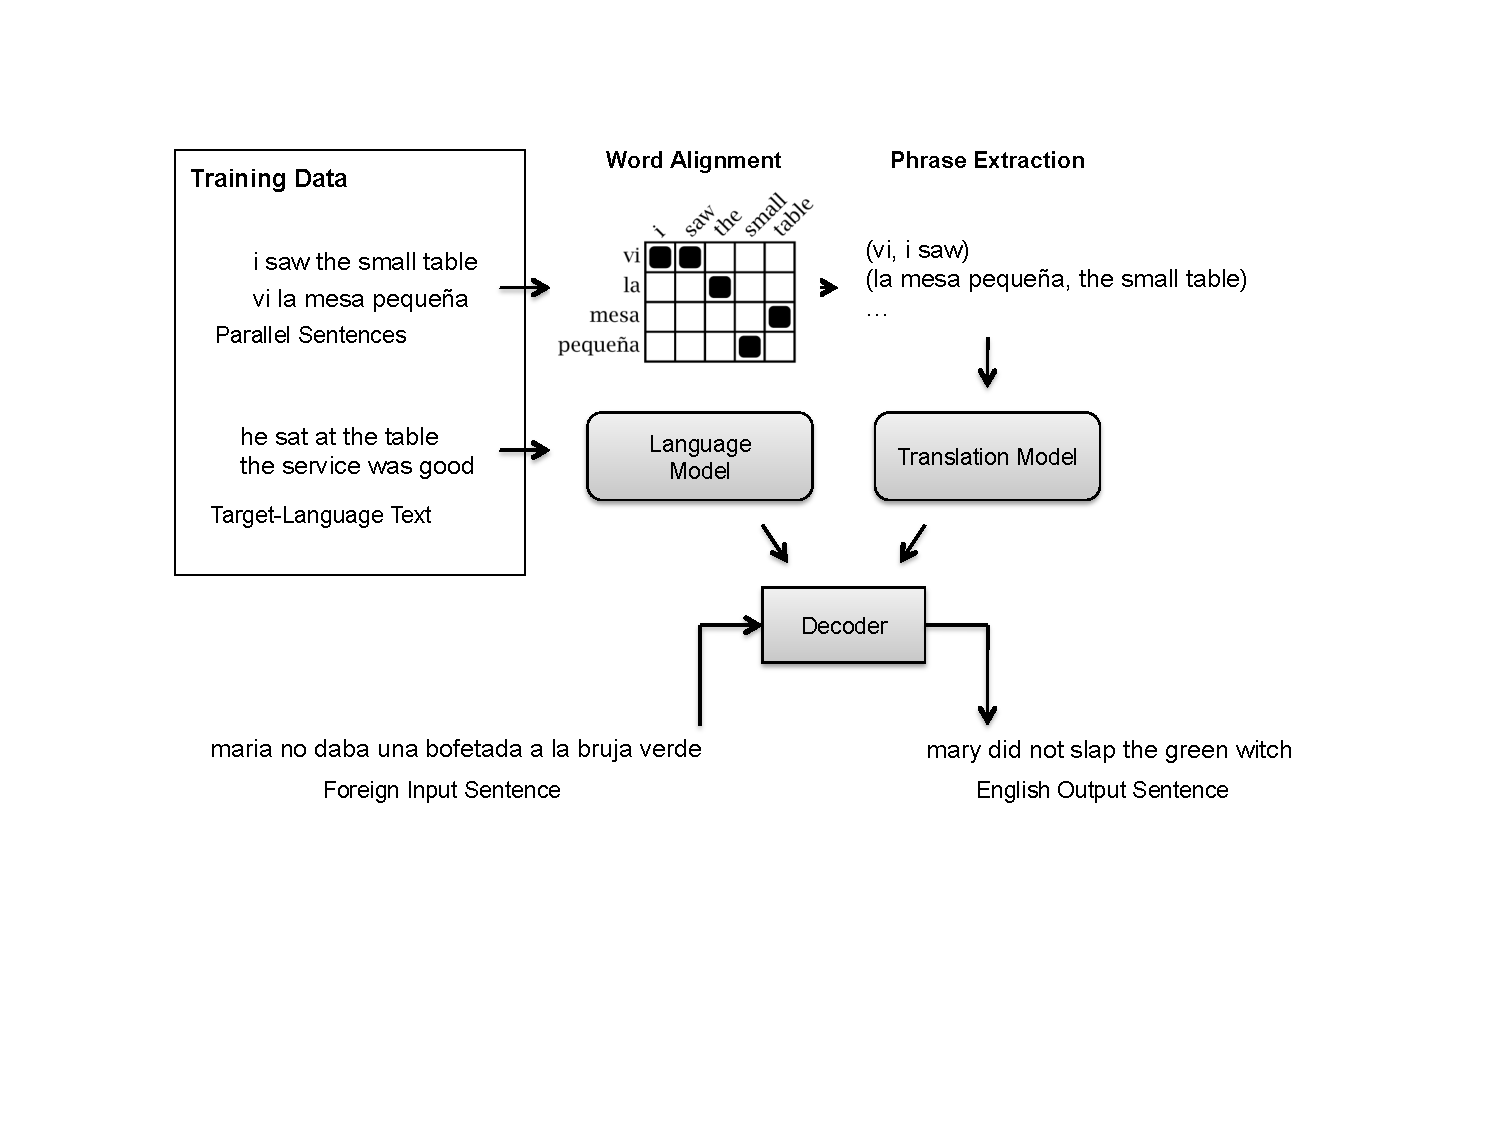
\includegraphics[scale=0.7]{figures/fig-ch6-MT-arch.pdf}
\end{center}\caption{The standard phrase-based machine translation architecture.  The translation model is constructed with phrases extracted from a word-aligned parallel corpus.  The language model is estimated from a monolingual corpus.  Both serve as input to the decoder, which performs the actual translation.}\label{chapter6_figure_mtarch}
\end{figure*}

\begin{figure*}[p]
\begin{center}
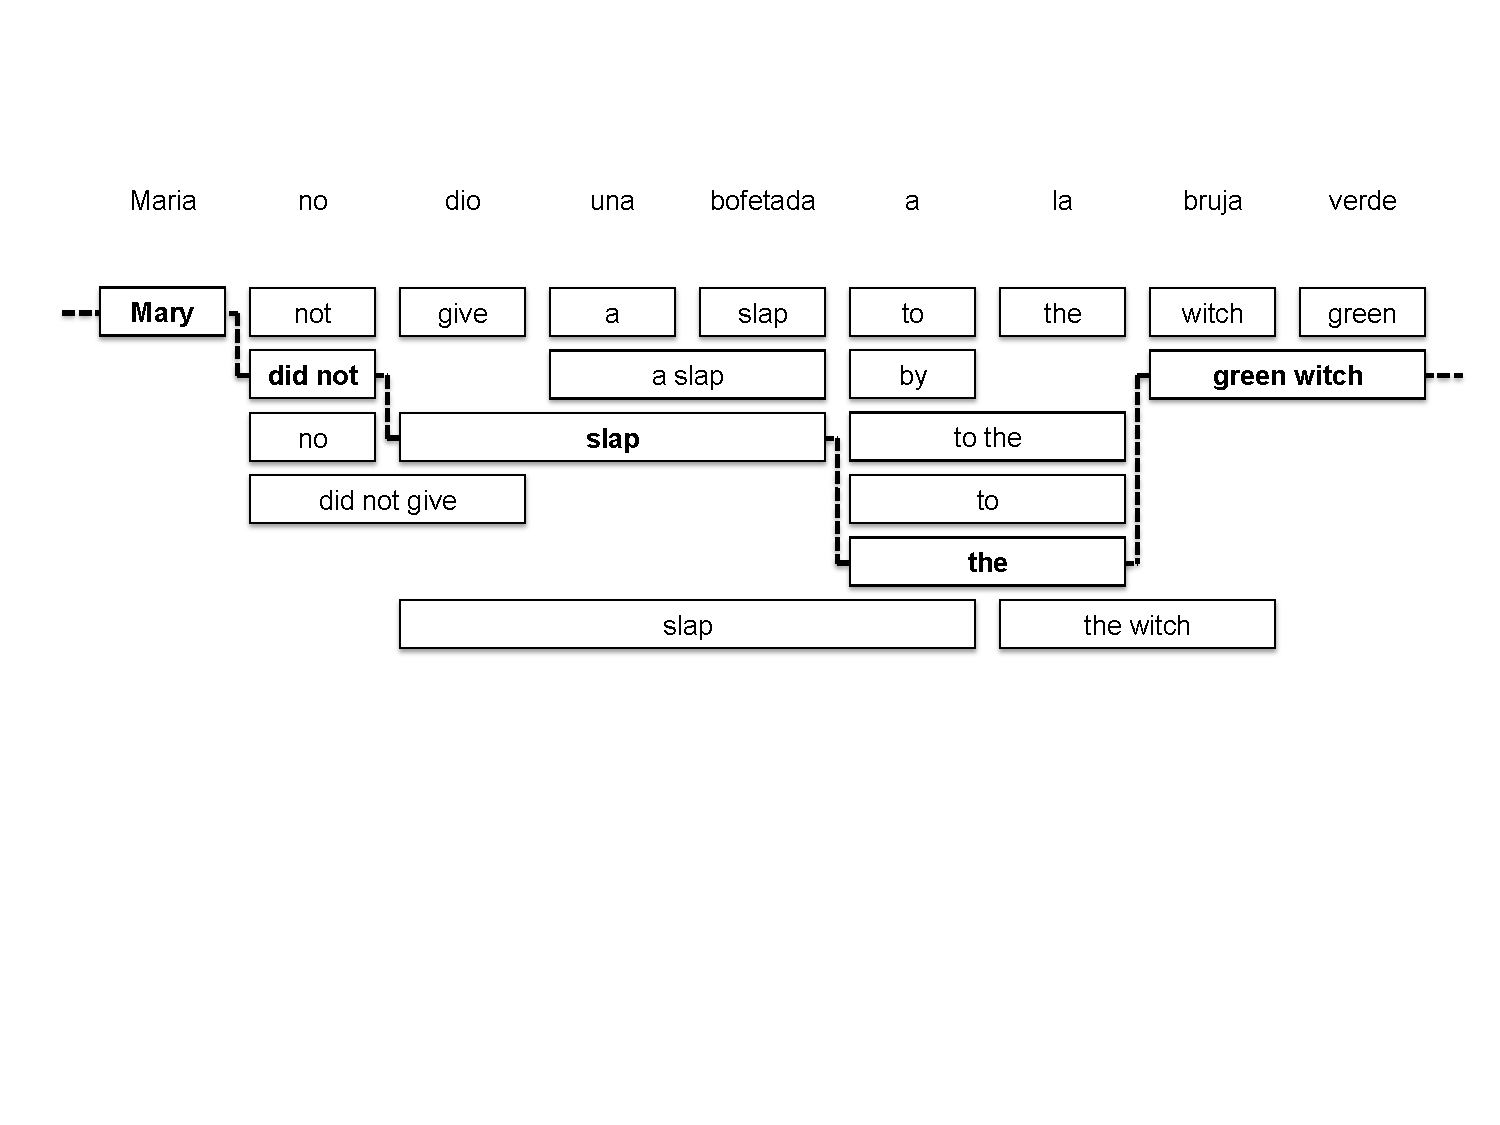
\includegraphics[scale=0.6]{figures/fig-ch6-MT-tiles.pdf}
\end{center}\caption{Translation coverage of the sentence \emph{Maria no dio una bofetada a la bruja verde} by a phrase-based model. The best possible translation path is indicated with a dashed line.}\label{chapter6_figure_mttiles}
\end{figure*}

A language model gives the probability that a string of words:
\begin{displaymath}
\textbf{w} = \langle w_1, w_2, \ldots , w_{n} \rangle, 
\end{displaymath}
written as
$w_{1}^{n}$ for short, is a string in the target language.  By the
chain rule of probability, we get:
\begin{align}
\Pr(w_{1}^{n}) &= \Pr(w_1) \Pr(w_2|w_1) \Pr(w_3|w_1^2) \ldots \Pr(w_n|w_1^{n-1}) \\
              &= \prod_{k=1}^{n} \Pr(w_k|w_1^{k-1})
\end{align}

\noindent Due to the extremely large number of parameters involved in
estimating such a model directly, it is customary to make the \emph{
  Markov assumption}, that the sequence histories only depend on prior
local context.  That is, an \emph{n}-gram language model is equivalent
to a ($n-1$)\emph{th}-order Markov model.  Thus, we can approximate
$P(w_k|w_1^{k-1})$ as follows:
\begin{align}
\textrm{bigrams:} & P(w_k|w_1^{k-1}) \approx P(w_k|w_{k-1}) \\
\textrm{trigrams:} & P(w_k|w_1^{k-1}) \approx P(w_k|w_{k-1} w_{k-2}) \\
\textrm{\emph{n}-grams:} & P(w_k|w_1^{k-1}) \approx  P(w_k|w_{k-n+1}^{k-1})
\end{align}

\noindent The probabilities used in computing $\Pr(w_{1}^{n})$ based
on an \emph{n}-gram language model are generally estimated from a
monolingual corpus of target language text.  Since only target
language text is necessary (without any additional annotation),
language modeling has been well served by large-data approaches that
take advantage of the vast quantities of text available on the web.

To translate an input sentence $\textbf{f}$, the phrase-based
\emph{decoder} creates a matrix of all translation possibilities of
all substrings in the input string, as an example illustrates in
Figure~\ref{chapter6_figure_mttiles}.  A sequence of phrase pairs is
selected such that each word in $\textbf{f}$ is translated exactly
once.\footnote{The phrases may not necessarily be selected in a strict
  left-to-right order.  Being able to vary the order of the phrases
  used is necessary since languages may express the same ideas using
  different word orders.}  The decoder seeks to find the translation
that maximizes the product of the translation probabilities of the
phrases used and the language model probability of the resulting
string in the target language.  Because the phrase translation
probabilities are independent of each other and the Markov assumption
made in the language model, this may be done efficiently using dynamic
programming.  For a detailed introduction to phrase-based decoding, we
refer the reader to a recent textbook by Koehn~\cite{Koehn_2009}.

\subsection{Brief Digression:\ Language Modeling with MapReduce}

Statistical machine translation provides the context for a brief
digression on distributed parameter estimation for language models
using MapReduce, and provides another example illustrating the
effectiveness data-driven approaches in general.  We briefly touched
upon this work in Chapter~\ref{chapter1}.  Even after making the
Markov assumption, training \emph{n}-gram language models still
requires estimating an enormous number of parameters:\ potentially
$V^n$, where $V$ is the number of words in the vocabulary.  For
higher-order models (e.g., 5-grams) used in real-world applications,
the number of parameters can easily exceed the number of words from
which to estimate those parameters.  In fact, most \emph{n}-grams will
never be observed in a corpus, no matter how large.  To cope with this
sparseness, researchers have developed a number of smoothing
techniques~\cite{Manning_Schutze_1999}, which all share the basic idea
of moving probability mass from observed to unseen events in a
principled manner.  For many applications, a state-of-the-art approach
is known as Kneser-Ney smoothing~\cite{Chen_Goodman_ACL1996}.

In 2007, Brants et al.~\cite{Brants_etal_EMNLP2007} reported
experimental results that answered an interesting question:\ given the
availability of large corpora (i.e., the web), could a simpler
smoothing strategy, applied to more text, beat Kneser-Ney in a machine
translation task?  It should come as no surprise that the answer is
\emph{yes}. Brants et al.\ introduced a technique known as ``stupid
backoff'' that was exceedingly simple and so na\"{i}ve that the
resulting model didn't even define a valid probability distribution
(it assigned arbitrary scores as opposed to probabilities).  The
simplicity, however, afforded an extremely scalable implementations in
MapReduce.  With smaller corpora, stupid backoff didn't work as well
as Kneser-Ney in generating accurate and fluent translations.
However, as the amount of data increased, the gap between stupid
backoff and Kneser-Ney narrowed, and eventually disappeared with
sufficient data.  Furthermore, with stupid backoff it was possible to
train a language model on more data than was feasible with Kneser-Ney
smoothing.  Applying this language model to a machine translation task
yielded better results than a (smaller) language model trained with
Kneser-Ney smoothing.

The role of the language model in statistical machine translation is
to select fluent, grammatical translations from a large hypothesis
space:\ the more training data a language model has access to, the
better its description of relevant language phenomena and hence its
ability to select good translations.  Once again, large data triumphs!
For more information about estimating language models using MapReduce,
we refer the reader to a forthcoming book from Morgan \&
Claypool~\cite{Brants_2010}.

\subsection{Word Alignment}

Word alignments, which are necessary for building phrase-based
translation models (as well as many other more sophisticated
translation models), can be learned automatically using EM.  In this
section, we introduce a popular alignment model based on HMMs.

In the statistical model of word alignment considered here, the
observable variables are the words in the source and target sentences
(conventionally written using the variables $\textbf{f}$ and
$\textbf{e}$, respectively), and their alignment is a latent variable.
To make this model tractable, we assume that words are translated
independently of one another, which means that the model's parameters
include the probability of any word in the source language translating
to any word in the target language.  While this independence
assumption is problematic in many ways, it results in a simple model
structure that admits efficient inference yet produces reasonable
alignments.  Alignment models that make this assumption generate a
string $\textbf{e}$ in the target language by selecting words in the
source language according to a lexical translation distribution.  The
indices of the words in $\textbf{f}$ used to generate each word in
$\textbf{e}$ are stored in an alignment variable,
$\textbf{a}$.\footnote{In the original presentation of statistical
  lexical translation models, a special null word is added to the
  source sentences, which permits words to be inserted `out of
  nowhere'.  Since this does not change any of the important details
  of training, we omit it from our presentation for simplicity.} This
means that the variable $a_i$ indicates the source word position of
the $i^{\textrm{\emph{th}}}$ target word generated, and $|\textbf{a}|
= |\textbf{e}|$.  Using these assumptions, the probability of an
alignment and translation can be written as follows:
\begin{align}
\Pr(\textbf{e}, \textbf{a} | \textbf{f}) =  \underbrace{  \Pr(\textbf{a} | \textbf{f} , \textbf{e}) }_{\textrm{Alignment probability}} \times  \underbrace{ \prod_{i=1}^{|\textbf{e}|} \Pr(e_i|f_{a_i}) }_{\textrm{Lexical probability}}
\end{align}

\noindent Since we have parallel corpora consisting of only $\langle
\textbf{f}, \textbf{e} \rangle$ pairs, we can learn the parameters for
this model using EM and treating $\textbf{a}$ as a latent variable.
However, to combat data sparsity in the alignment probability, we must
make some further simplifying assumptions.  By letting the probability
of an alignment depend only on the position of the previous aligned
word we capture a valuable insight (namely, words that are nearby in
the source language will tend to be nearby in the target language),
and our model acquires the structure of an HMM \cite{Vogel_1996}:
\begin{align}
\Pr(\textbf{e}, \textbf{a} | \textbf{f}) = \underbrace{\prod_{i=1}^{|\textbf{e}|} \Pr(a_i | a_{i-1})}_{\textrm{Transition probability}} \times \underbrace{\prod_{i=1}^{|\textbf{e}|} \Pr(e_i|f_{a_i})}_{\textrm{Emission probability}} 
\end{align}

\noindent This model can be trained using the forward-backward
algorithm described in the previous section, summing over all settings
of $\textbf{a}$, and the best alignment for a sentence pair can be
found using the Viterbi algorithm.

To properly initialize this HMM, it is conventional to further
simplify the alignment probability model, and use this simpler model
to learn initial lexical translation (emission) parameters for the
HMM.  The favored simplification is to assert that all alignments are
uniformly probable:
\begin{align}
\Pr(\textbf{e}, \textbf{a} | \textbf{f}) = \frac{1}{|\textbf{f}|^{|\textbf{e}|}} \times \prod_{i=1}^{|\textbf{e}|} \Pr(e_i|f_{a_i}) 
\end{align}

\noindent This model is known as IBM Model 1.  It is attractive for
initialization because it is convex everywhere, and therefore EM will
learn the same solution regardless of initialization.  Finally, while
the forward-backward algorithm could be used to compute the expected
counts necessary for training this model by setting $A_q(r)$ to be a
constant value for all $q$ and $r$, the uniformity assumption means
that the expected emission counts can be estimated in time
$O(|\textbf{e}| \cdot |\textbf{f}|)$, rather than time $O(|\textbf{e}|
\cdot |\textbf{f}|^2)$ required by the forward-backward algorithm.

\subsection{Experiments}

How well does a MapReduce word aligner for statistical machine
translation perform?  We describe previously-published
results~\cite{Dyer_etal_2008} that compared a Java-based Hadoop
implementation against a highly optimized word aligner called
Giza++~\cite{Och_2003}, which was written in C++ and designed to run
efficiently on a single core.  We compared the training time of Giza++
and our aligner on a Hadoop cluster with 19 slave nodes, each with two
single-core processors and two disks (38 cores total).

Figure~\ref{chapter6_figure_giza_timing} shows the performance of
Giza++ in terms of the running time of a single EM iteration for both
Model 1 and the HMM alignment model as a function of the number of
training pairs.  Both axes in the figure are on a log scale, but the
ticks on the $y$-axis are aligned with `meaningful' time intervals
rather than exact orders of magnitude.  There are three things to
note.  First, the running time scales linearly with the size of the
training data.  Second, the HMM is a constant factor slower than Model
1.  Third, the alignment process is quite slow as the size of the
training data grows---at one million sentences, a single iteration
takes over three hours to complete!  Five iterations are generally
necessary to train the models, which means that full training takes
the better part of a day.

In Figure~\ref{chapter6_figure_mr_timing} we plot the running time of
our MapReduce implementation running on the 38-core cluster described
above.  For reference, we plot points indicating what 1/38 of the
running time of the Giza++ iterations would be at each data size,
which gives a rough indication of what an `ideal' parallelization
could achieve, assuming that there was no overhead associated with
distributing computation across these machines.  Three things may be
observed in the results.  First, as the amount of data increases, the
relative cost of the overhead associated with distributing data,
marshaling and aggregating counts, decreases.  At one million sentence
pairs of training data, the HMM alignment iterations begin to approach
optimal runtime efficiency.  Second, Model 1, which we observe is
light on computation, does not approach the theoretical performance of
an ideal parallelization, and in fact, has almost the same running
time as the HMM alignment algorithm. We conclude that the overhead
associated with distributing and aggregating data is significant
compared to the Model 1 computations, although a comparison with
Figure~\ref{chapter6_figure_giza_timing} indicates that the MapReduce
implementation is still substantially faster than the single core
implementation, at least once a certain training data size is reached.
Finally, we note that, in comparison to the running times of the
single-core implementation, at large data sizes, there is a
significant advantage to using the distributed implementation, even of
Model 1.

Although these results do confound several variables (Java vs. C++
performance, memory usage patterns), it is reasonable to expect that
the confounds would tend to make the single-core system's performance
appear relatively \emph{better} than the MapReduce system (which is,
of course, the opposite pattern from what we actually observe).
Furthermore, these results show that when computation is distributed
over a cluster of many machines, even an unsophisticated
implementation of the HMM aligner could compete favorably with a
highly optimized single-core system whose performance is well-known to
many people in the MT research community.

\begin{figure*}[p]
\begin{center}
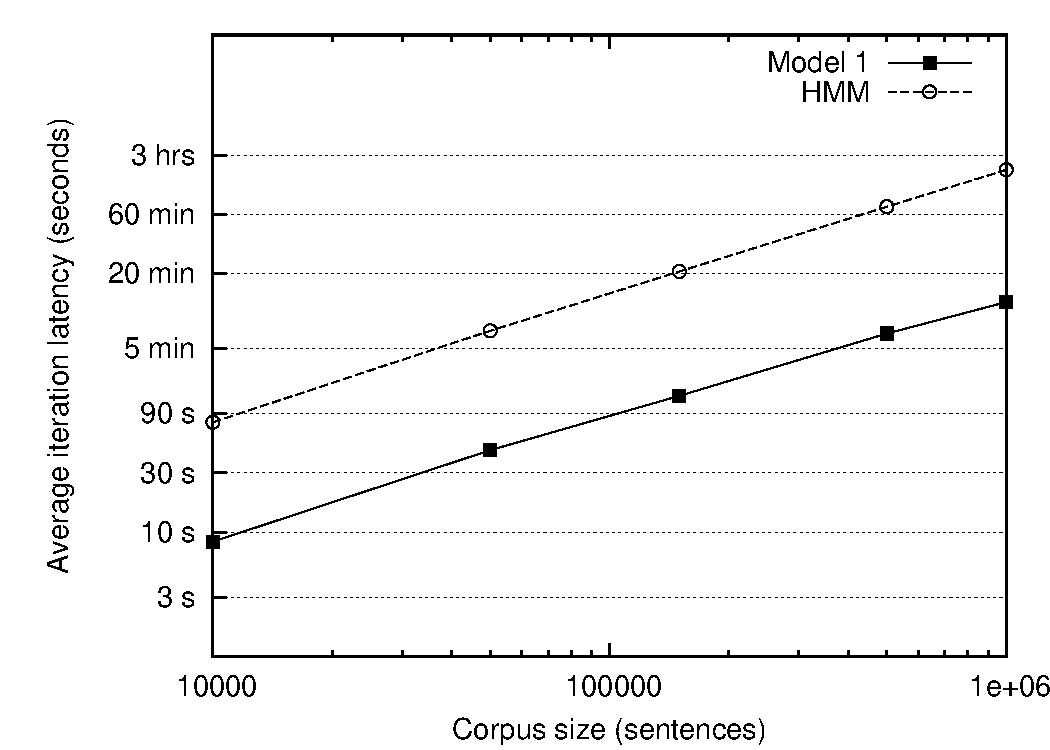
\includegraphics[scale=0.6]{figures/fig-ch6-GIZA-timing.pdf}
\end{center}\caption{Running times of Giza++ (baseline single-core system) for Model 1 and HMM training iterations at various corpus sizes.}\label{chapter6_figure_giza_timing}
\end{figure*}

\begin{figure*}[p]
\begin{center}
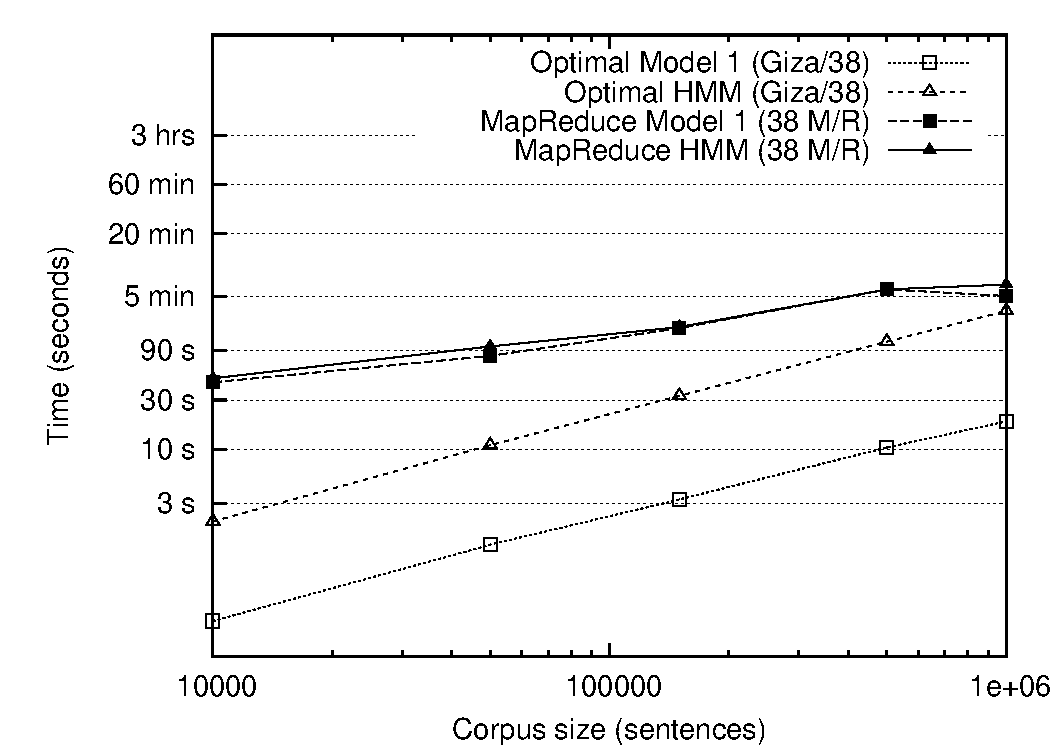
\includegraphics[scale=0.6]{figures/fig-ch6-alignment-timing.pdf}
\end{center}\caption{Running times of our MapReduce implementation of Model 1 and HMM training iterations at various corpus sizes.  For reference, $1/38$ running times of the Giza++ models are shown.}\label{chapter6_figure_mr_timing}
\end{figure*}

Why are these results important? Perhaps the most significant reason
is that the quantity of parallel data that is available to train
statistical machine translation models is ever increasing, and as is
the case with so many problems we have encountered, more data leads to
improvements in translation quality \cite{Dyer_etal_2008}.  Recently a
corpus of one billion words of French-English data was mined
automatically from the web and released publicly
\cite{Callison_Burch_2009}.\footnote{\texttt{
    http://www.statmt.org/wmt10/translation-task.html}} Single-core
solutions to model construction simply cannot keep pace with the
amount of translated data that is constantly being
produced. Fortunately, several independent researchers have shown that
existing modeling algorithms can be expressed naturally and
effectively using MapReduce, which means that we can take advantage of
this data.  Furthermore, the results presented here show that even at
data sizes that may be tractable on single machines, significant
performance improvements are attainable using MapReduce
implementations.  This improvement reduces experimental turnaround
times, which allows researchers to more quickly explore the solution
space---which will, we hope, lead to rapid new developments in
statistical machine translation.

For the reader interested in statistical machine translation, there is
an open source Hadoop-based MapReduce implementation of a training
pipeline for phrase-based translation that includes word alignment,
phrase extraction, and phrase scoring \cite{Gao_2010}.

\section{EM-Like Algorithms}
\label{chapter6_variants}

This chapter has focused on expectation maximization algorithms and
their implementation in the MapReduce programming framework.  These
important algorithms are indispensable for learning models with latent
structure from unannotated data, and they can be implemented quite
naturally in MapReduce.  We now explore some related learning
algorithms that are similar to EM but can be used to solve more
general problems, and discuss their implementation.

In this section we focus on \emph{gradient-based optimization}, which
refers to a class of techniques used to optimize any objective
function, provided it is differentiable with respect to the parameters
being optimized.  Gradient-based optimization is particularly useful
in the learning of maximum entropy (maxent) models~\cite{Nigam_1999}
and conditional random fields (CRF)~\cite{Lafferty_2001} that have an
exponential form and are trained to maximize conditional likelihood.
In addition to being widely used supervised classification models in
text processing (meaning that during training, both the data and their
annotations must be observable), their gradients take the form of
expectations.  As a result, some of the previously-introduced
techniques are also applicable for optimizing these models.

\subsection{Gradient-Based Optimization and Log-Linear Models}

Gradient-based optimization refers to a class of iterative
optimization algorithms that use the derivatives of a function to find
the parameters that yield a minimal or maximal value of that function.
Obviously, these algorithms are only applicable in cases where a
useful objective exists, is differentiable, and its derivatives can be
efficiently evaluated.  Fortunately, this is the case for many
important problems of interest in text processing.  For the purposes
of this discussion, we will give examples in terms of minimizing
functions.

Assume that we have some real-valued function $F(\theta)$ where
$\theta$ is a $k$-dimensional vector and that $F$ is differentiable
with respect to $\theta$.  Its gradient is defined as:
\begin{equation}
\nabla F(\theta) = \left\langle \frac{\partial F}{\partial \theta_1}(\theta), \frac{\partial F}{\partial \theta_2}(\theta) , \ldots , \frac{\partial F}{\partial \theta_k}(\theta) \right\rangle
\end{equation}

\noindent The gradient has two crucial properties that are exploited
in gradient-based optimization.  First, the gradient $\nabla F$ is a
vector field that points in the direction of the greatest increase of
$F$ and whose magnitude indicates the rate of increase.  Second, if
$\theta^*$ is a (local) minimum of F, then the following is true:
\begin{equation}
\nabla F(\theta^*) = 0
\end{equation}

An extremely simple gradient-based minimization algorithm produces a
series of parameter estimates $\theta^{(1)}, \theta^{(2)}, \ldots$ by
starting with some initial parameter settings $\theta^{(1)}$ and
updating parameters through successive iterations according to the
following rule:
\begin{equation}
\theta^{(i+1)} = \theta^{(i)} - \eta^{(i)} \nabla F(\theta^{(i)})
\label{chapter6_eq_grad_opt1}
\end{equation}

\noindent The parameter $\eta^{(i)} > 0$ is a learning rate which
indicates how quickly the algorithm moves along the gradient during
iteration $i$.  Provided this value is small enough that $F$
decreases, this strategy will find a local minimum of $F$.  However,
while simple, this update strategy may converge slowly, and proper
selection of $\eta$ is non-trivial.  More sophisticated algorithms
perform updates that are informed by approximations of the second
derivative, which are estimated by successive evaluations of $\nabla
F(\theta)$, and can converge much more rapidly \cite{LBFGS}.

\paragraph{\textbf{Gradient-based optimization in MapReduce.}}
Gradient-based optimization algorithms can often be implemented
effectively in MapReduce.  Like EM, where the structure of the model
determines the specifics of the realization, the details of the
function being optimized determines how it should best be implemented,
and not every function optimization problem will be a good fit for
MapReduce.  Nevertheless, MapReduce implementations of gradient-based
optimization tend to have the following characteristics:

\begin{itemize}

\item Each optimization iteration is one MapReduce job.

\item The objective should decompose linearly across training
  instances.  This implies that the gradient also decomposes linearly,
  and therefore mappers can process input data in parallel.  The
  values they emit are pairs $\langle F(\theta), \nabla F(\theta)
  \rangle$, which are linear components of the objective and gradient.

\item Evaluation of the function and its gradient is often
  computationally expensive because they require processing lots of
  data.  This make parallelization with MapReduce worthwhile.

\item Whether more than one reducer can run in parallel depends on the
  specific optimization algorithm being used.  Some, like the trivial
  algorithm of Equation~\ref{chapter6_eq_grad_opt1} treat the
  dimensions of $\theta$ independently, whereas many are sensitive to
  global properties of $\nabla F(\theta)$.  In the latter case,
  parallelization across multiple reducers is non-trivial.

\item Reducer(s) sum the component objective/gradient pairs, compute
  the total objective and gradient, run the optimization algorithm,
  and emit $\theta^{(i+1)}$.

\item Many optimization algorithms are stateful and must persist their
  state between optimization iterations.  This may either be emitted
  together with $\theta^{(i+1)}$ or written to the distributed file
  system as a side effect of the reducer. Such external side effects
  must be handled carefully; refer to
  Section~\ref{chapter2:mappers-and-reducers} for a discussion.

\end{itemize}


\paragraph{\textbf{Parameter learning for log-linear models.}}
Gradient-based optimization techniques can be quite effectively used
to learn the parameters of probabilistic models with a log-linear
parameterization \cite{Malouf_2002}.  While a comprehensive
introduction to these models is beyond the scope of this book, such
models are used extensively in text processing applications, and their
training using gradient-based optimization, which may otherwise be
computationally expensive, can be implemented effectively using
MapReduce. We therefore include a brief summary.

Log-linear models are particularly useful for supervised learning
(unlike the unsupervised models learned with EM), where an annotation
$\textbf{y} \in \mathcal{Y}$ is available for every $\textbf{x} \in
\mathcal{X}$ in the training data.  In this case, it is possible to
directly model the conditional distribution of label given input:
\begin{equation}
\Pr(\textbf{y} | \textbf{x} ; \theta) = \frac{\exp \sum_i \theta_i \cdot H_i(\textbf{x}, \textbf{y})}{\sum_{\textbf{y}'}\exp \sum_i \theta_i \cdot H_i(\textbf{x}, \textbf{y}')}
\end{equation}

\noindent In this expression, $H_i$ are real-valued functions
sensitive to features of the input and labeling.  The parameters of
the model is selected so as to minimize the negative conditional log
likelihood of a set of training instances $\langle \langle \textbf{x}
, \textbf{y} \rangle_1 , \langle \textbf{x} , \textbf{y} \rangle_2 ,
\ldots \rangle$, which we assume to be i.i.d.:
\begin{align}
F(\theta) & = \sum_{\langle \textbf{x} , \textbf{y} \rangle} - \log \Pr(\textbf{y} | \textbf{x} ; \theta) \label{chapter6_eq_meobj} \\
\theta^* & = \arg \min_\theta F(\theta)
\end{align}

\noindent As Equation~\ref{chapter6_eq_meobj} makes clear, the
objective decomposes linearly across training instances, meaning it
can be optimized quite well in MapReduce.  The gradient derivative of
$F$ with respect to $\theta_i$ can be shown to have the following form
\cite{Smith_2004}:\footnote{This assumes that when $\langle
  \textbf{x}, \textbf{y} \rangle$ is present the model is fully
  observed (i.e., there are no additional latent variables).}
\begin{equation}
\frac{\partial F}{\partial \theta_i}(\theta) = \sum_{\langle \textbf{x} , \textbf{y} \rangle} \left[ H_i(\textbf{x},\textbf{y}) - \mathbb{E}_{\Pr(\textbf{y}' | \textbf{x} ; \theta)}[H_i(\textbf{x},\textbf{y}')] \right]
\end{equation}

\noindent The expectation in the second part of the gradient's
expression can be computed using a variety of techniques.  However, as
we saw with EM, when very large event spaces are being modeled, as is
the case with sequence labeling, enumerating all possible values
$\textbf{y}$ can become computationally intractable.  And, as was the
case with HMMs, independence assumptions can be used to enable
efficient computation using dynamic programming.  In fact, the
forward-backward algorithm introduced in
Section~\ref{chapter6_forward_backward} can, with only minimal
modification, be used to compute the expectation
$\mathbb{E}_{\Pr(\textbf{y}' | \textbf{x} ;
  \theta)}[H_i(\textbf{x},\textbf{y}')]$ needed in CRF sequence
models, as long as the feature functions respect the same Markov
assumption that is made in HMMs.  For more information about inference
in CRFs using the forward-backward algorithm, we refer the reader to
Sha et al.~\cite{Sha_2003}.

As we saw in the previous section, MapReduce offers significant
speedups when training iterations require running the forward-backward
algorithm.  The same pattern of results holds when training linear
CRFs.

\section{Summary and Additional Readings}
\label{chapter6_conclusions}

This chapter focused on learning the parameters of statistical models
from data, using expectation maximization algorithms or gradient-based
optimization techniques.  We focused especially on EM algorithms for
three reasons.  First, these algorithms can be expressed naturally in
the MapReduce programming model, making them a good example of how to
express a commonly-used algorithm in this new framework.  Second, many
models, such as the widely-used hidden Markov model (HMM) trained
using EM, make independence assumptions that permit an high degree of
parallelism in both the E- and M-steps.  Thus, they are particularly
well-positioned to take advantage of large clusters.  Finally, EM
algorithms are unsupervised learning algorithms, which means that they
have access to far more training data than comparable supervised
approaches.  This is quite important.  In Chapter~\ref{chapter1}, when
we hailed large data as the ``rising tide that lifts all boats'' to
yield more effective algorithms, we were mostly referring to
unsupervised approaches, given that the manual effort required to
generate annotated data remains a bottleneck in many supervised
approaches.  Data acquisition for unsupervised algorithms is often as
simple as crawling specific web sources, given the enormous quantities
of data available ``for free''.  This, combined with the ability of
MapReduce to process large datasets in parallel, provides researchers
with an effective strategy for developing increasingly-effective
applications.

Since EM algorithms are relatively computationally expensive, even for
small amounts of data, this led us to consider how related supervised
learning models (which typically have much less training data
available), can also be implemented in MapReduce.  The discussion
demonstrates that not only does MapReduce provide a means for coping
with ever-increasing amounts of data, but it is also useful for
parallelizing expensive computations.  Although MapReduce has been
designed with mostly data-intensive applications in mind, the ability
to leverage clusters of commodity hardware to parallelize
computationally-expensive algorithms is an important use case.

\paragraph{Additional Readings.}
Because of its ability to leverage large amounts of training data,
machine learning is an attractive problem for MapReduce and an area of
active research.  Chu et al.~\cite{ChuCT_etal_2006} presented general
formulations of a variety of machine learning problems, focusing on a
normal form for expressing a variety of machine learning algorithms in
MapReduce.  The Apache Mahout project is an open-source implementation
of these and other learning algorithms,\footnote{\texttt{
  http://lucene.apache.org/mahout/}} and it is also the subject of a
forthcoming book~\cite{Owen_2010}.  Issues associated with a MapReduce
implementation of latent Dirichlet allocation (LDA), which is another
important unsupervised learning technique, with certain similarities
to EM, have been explored by Wang et al.~\cite{WangYi_etal_2009}.
